\chapter{Modelling the deformation of solid objects in real-time}
\label{chap4}
\begin{shortAbstract}
Modelling the deformation of solid organs is a crucial problem in medical simulation. If the finite element method is classicaly used in mechanical engineering for its ability to solve the equations of continuum mechanics fairly accurately, its development in medical simulation was more progressive. The main reason for this is that the finite element method is computationally demanding and not easily compatible with time constraints required in interactive simulation. Therefore, other methods were developed to allow faster computations, at the cost of larger approximations of course. Over time, along with the increase in computational power, methods became more elaborate and less approximative. These different approaches may be grouped into three main categories: (1) geometrically based techniques, (2) approaches physically motivated and (3) methods actually based on the equations of continuum mechanics. In this chapter, we will review the most classic methods applied to modelling of solid objects with a particular emphasis on medical simulation. 
\end{shortAbstract}


\section{Introduction: the problematic}

At the beginning of computer simulation, users were immersed into environments that were merely a decor. If it could virtually take the user somewhere else, a static scene quickly showed its limits. Indeed, in a real-life environment many objects are in motion, interacting with each others. Therefore, in order to increase the fidelity of simulations, elements of physics were progressively added. It could be as simple as adding motion to clouds in a flight simulator for instance. But by improving the dynamism of the scene, the simulation appears more natural to users. Over time, with the increase of computers' computational power, objects stopped being all rigid and simulators started taking laws of physics into account. In other words, objects became deformable. If this took the realism a step further, the demands in computational power were multiplied. Simulators eventually faced a challenge: they had to weight the desired degree of realism against the computational power at their disposal. 

In the field of medical simulation, the correctness of deformation is often crucial. This is particulary true in the cases of per-operative guidance. As an example, removing a brain tumor relies heavily on knowing the spatial relation between the patient's brain and the images acquired prior to surgery. Unfortunately, drilling a hole into the patient's skull releases pressure and the brain deforms. This phenomenon is called brain shift. The overall deformation is quite complex and the displacements depend on local elasticity of the brain, the size and the location of the tumor. A large brain shift, if not corrected, will result in inaccuracies in the surgical procedure and has the potential to cause damage to normal tissue. A solution is to accurately model the mechanical response of the patient's brain to predict the actual deformation and hence keep the knowledge of the tumor's location. 

Conversely, when medical simulation is applied to training, such a precision in terms of distance is not required. The physician would not even visually notice reasonable errors as soon as it looks realistic enough. However, in some medical procedures, the sense of touch and the forces that the physician can feel are a fey factor for the success of the operation. For instance, during a colonoscopy procedure, force feedback gives precious information about what type of loop is forming and the physician can then react accordingly to prevent loop formation. Consequently, a good colonoscopy simulator is required to provide accurate force feedbacks. If the contact forces were not reproduced to the operator, he would never be able to learn how to detect loop forming. Obviously, the computation of a realistic force to be returned demands an appropriate mechanical modelling of all structures. 

If the reasons differ, the need for modelling the mechanical response of organs with precision remains. However, strong time constraints often limit the complexity of the modelling and affects the overall accuracy. Because of this trade-off, various approaches were proposed over the years to fit into real-time constraints and may be grouped into three main categories: (1) geometrically based techniques, (2) approaches physically motivated (usually relying on Newton's second law) and (3) methods actually based on the equations of continuum mechanics. 



\section{Techniques based on geometry}

	\subsection{Free-form deformation}
The first needs to deforming solid objects came from for the field of solid modelling. The goal was to allow the designer to shape an object into the form he wishes in a similar way that clay is manipulated by a sculptor's hands. \cite{Sederberg86} introduced a technique called \emph{free-form deformation} based on the paper of \cite{Barr84}. It involves a mapping from $ \field{R}^3 $ to $ \field{R}^3 $ through a tensor product trivariate Bernstein polynomial. The deformed shape of the object is interpolated using control points as in the case of B�zier curves and surface patches (see \fig{chap4:fig-cubeFFD}). 
%
\begin{figure}[h]
\begin{center}
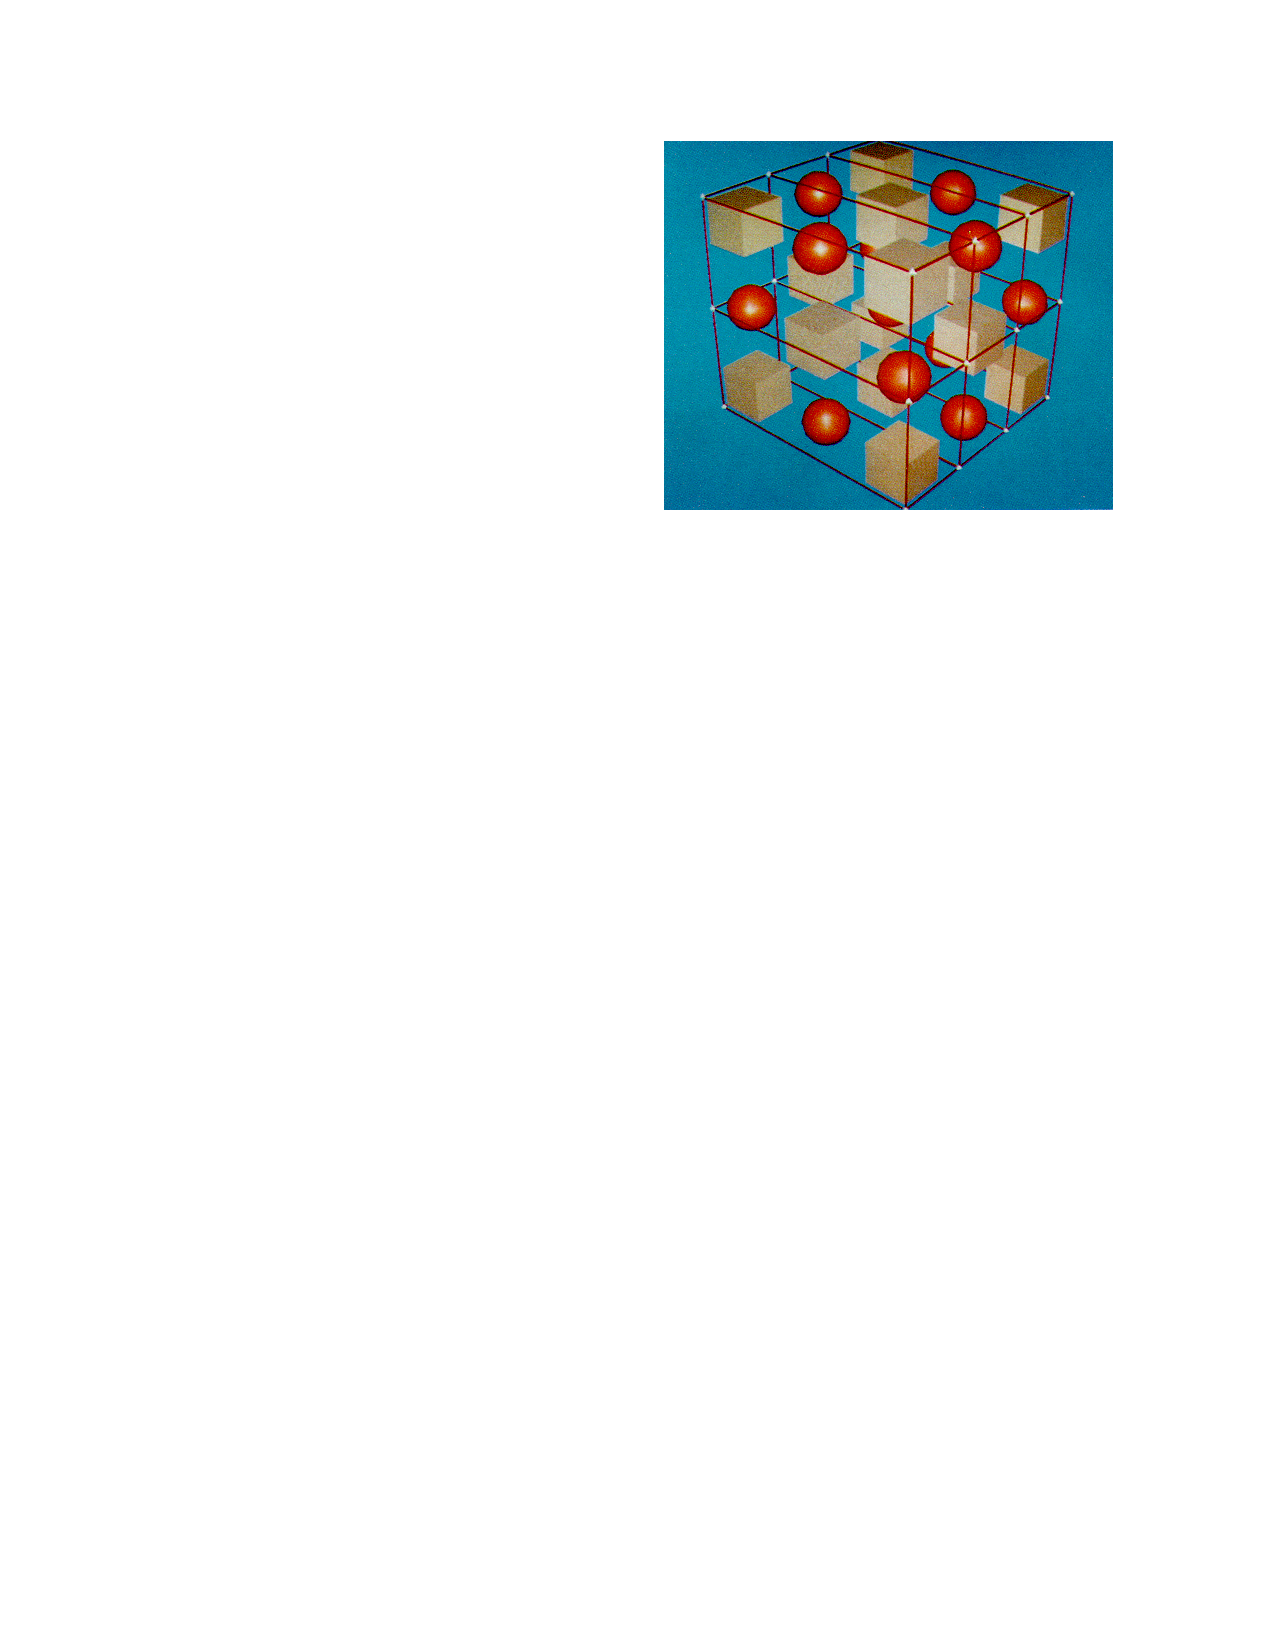
\includegraphics[width=6.5cm]{chapter4/cubeFFD1.pdf}
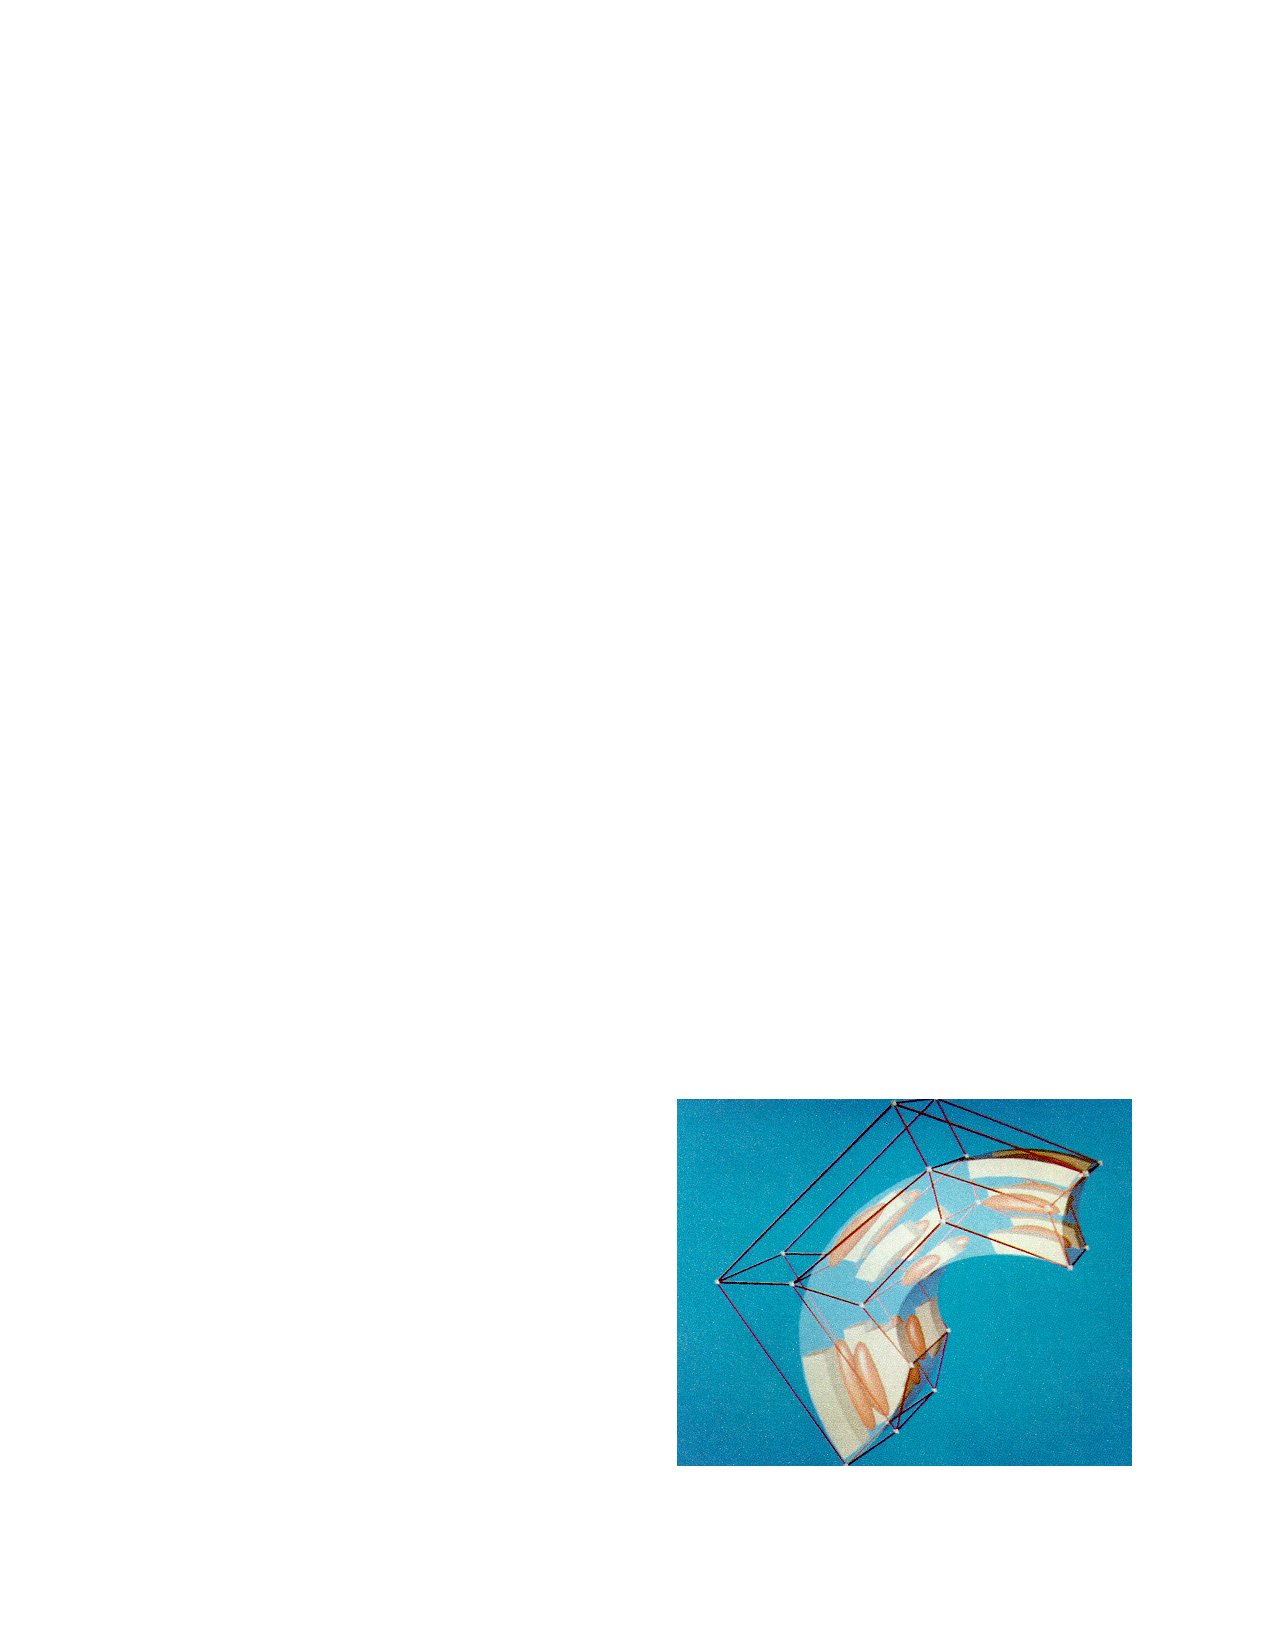
\includegraphics[width=6.6cm]{chapter4/cubeFFD2.pdf}
\end{center}
\caption[Deformation of objects by free-form deformation]{Let us imagine that the objects that we want to deform (spheres and cubes) are placed into a transparent parallelepiped \textbf{(left)}. Control points are indicated by small white diamonds. The free-form deformation technique offers to compute the deformation of the objects from the positions of the control points \textbf{(right)}.}
\label{chap4:fig-cubeFFD}
\end{figure}
The capability of locally applying deformations makes the technique strongly analogous to sculpting with clay, which was the sought target. Although the authors do not give details on computational efficiency, their work constitutes the beginnings of deformable solid objects. 

Coquillard later developed the idea of Extented free-form deformation \citeyearpar{Coquillart90} and Animated free-form technique \citeyearpar{Coquillart91}. The idea of free-form deformation with lattices of arbitrary topology was introduced by \cite{MacCracken96}. Finally, \cite{Schein04} presented a technique to facilitate the incorporation of discontinuities in a model while deforming it. 


	
	\subsection{Shape matching}
One field particulary interested in modelling deformable objects in a very efficient way is the game industry. Of course, for games we are more attracted by computational efficiency and extreme stability features than accuracy to physics laws. Most of the time, we can tolerate a degradation of realism as long as the result looks realistic. \cite{Muller05} developed a technique with this idea in mind called \emph{shape matching}. We start with a set of particules with masses $ m_i $ in an initial configuration where we denote by $ \mathbf{x}_i^0 $ the initial positions of the particules. No connectivity information is required. The particles are simulated as a simple particle system without particle-particle interactions, but including response to collisions with the environment and including external forces such as gravity. The positions in the deformed configuration are noted $ \mathbf{x}_i $. The method consists of finding a set of points $ \mathbf{g}_i $ which minimises the difference between the two sets $ \mathbf{x}_i^0 $ and $ \mathbf{x}_i $. The first step is to find the rotation matrix $ \mathbf{R} $ and the translation vectors $ \mathbf{t} $ and $ \mathbf{t}_0 $ such that
\begin{equation}
\sum_i m_i (\mathbf{R}(\mathbf{x}_i^0 - \mathbf{t}_0) + \mathbf{t} - \mathbf{x}_i)^2
\end{equation}
is minimal. The optimal translation vectors $ \mathbf{t} $ and $ \mathbf{t}_0 $ turn out to be the centre of mass of the initial shape and actual shape, that we will note $ \mathbf{x}_{c}^0 $ and $ \mathbf{x}_c $, respectively. The optimal rotation matrix is found by first finding the optimal linear transformation $ \mathbf{A} $. The optimal rotation is eventually obtained through the rotational part of $ \mathbf{A} $ after a polar decomposition. Finally, the goal positions $ \mathbf{g}_i $ can be computed as follows:
\begin{equation}
\label{chap4:gi}
\mathbf{g}_i = \mathbf{R}(\mathbf{x}_i^0 - \mathbf{x}_{c}^0) + \mathbf{x}_{c}.
\end{equation}
Once the goal positions are known, they are used to integrate the positions of the particules:
\begin{equation}  
	\begin{cases} 
		\mathbf{v}_i(t+h) = \mathbf{v}_i(t) + \alpha \dfrac{\mathbf{g}_i(t) - \mathbf{x}_i(t)}{h}  + h \dfrac{f_{\text{ext}}(t)}{m_i} \\\\
		\mathbf{x}_i(t+h) = \mathbf{x}_i(t) + h \mathbf{v}_i(t+h)
	\end{cases}
\end{equation}
where $ \alpha $ is a parameter between $ 0 $ and $ 1 $ which simulates stiffness. Because the method in this basic form is not suitable for objects undergoing large deformations, it is then extended to linear and quadratic deformations by replacing $ \mathbf{R} $ in \eqref{chap4:gi} with combinations of the form $ \beta \mathbf{A} + (1-\beta) \mathbf{R}$ where $ \beta $ is an additional parameter. Linear transformation can represent shear and stretch while quadratic transformation add twist and bending. Of course, this technique is not physically realistic. But this is beyond the point. This method allows the authors to simulate hundreds of deformable objects at an interactive rate with an unconditional stability (see \fig{chap4:fig-shoes}). Another illustration of this stability is shown \fig{chap4:fig-duck}. 
%
\begin{figure}[h]
\begin{center}
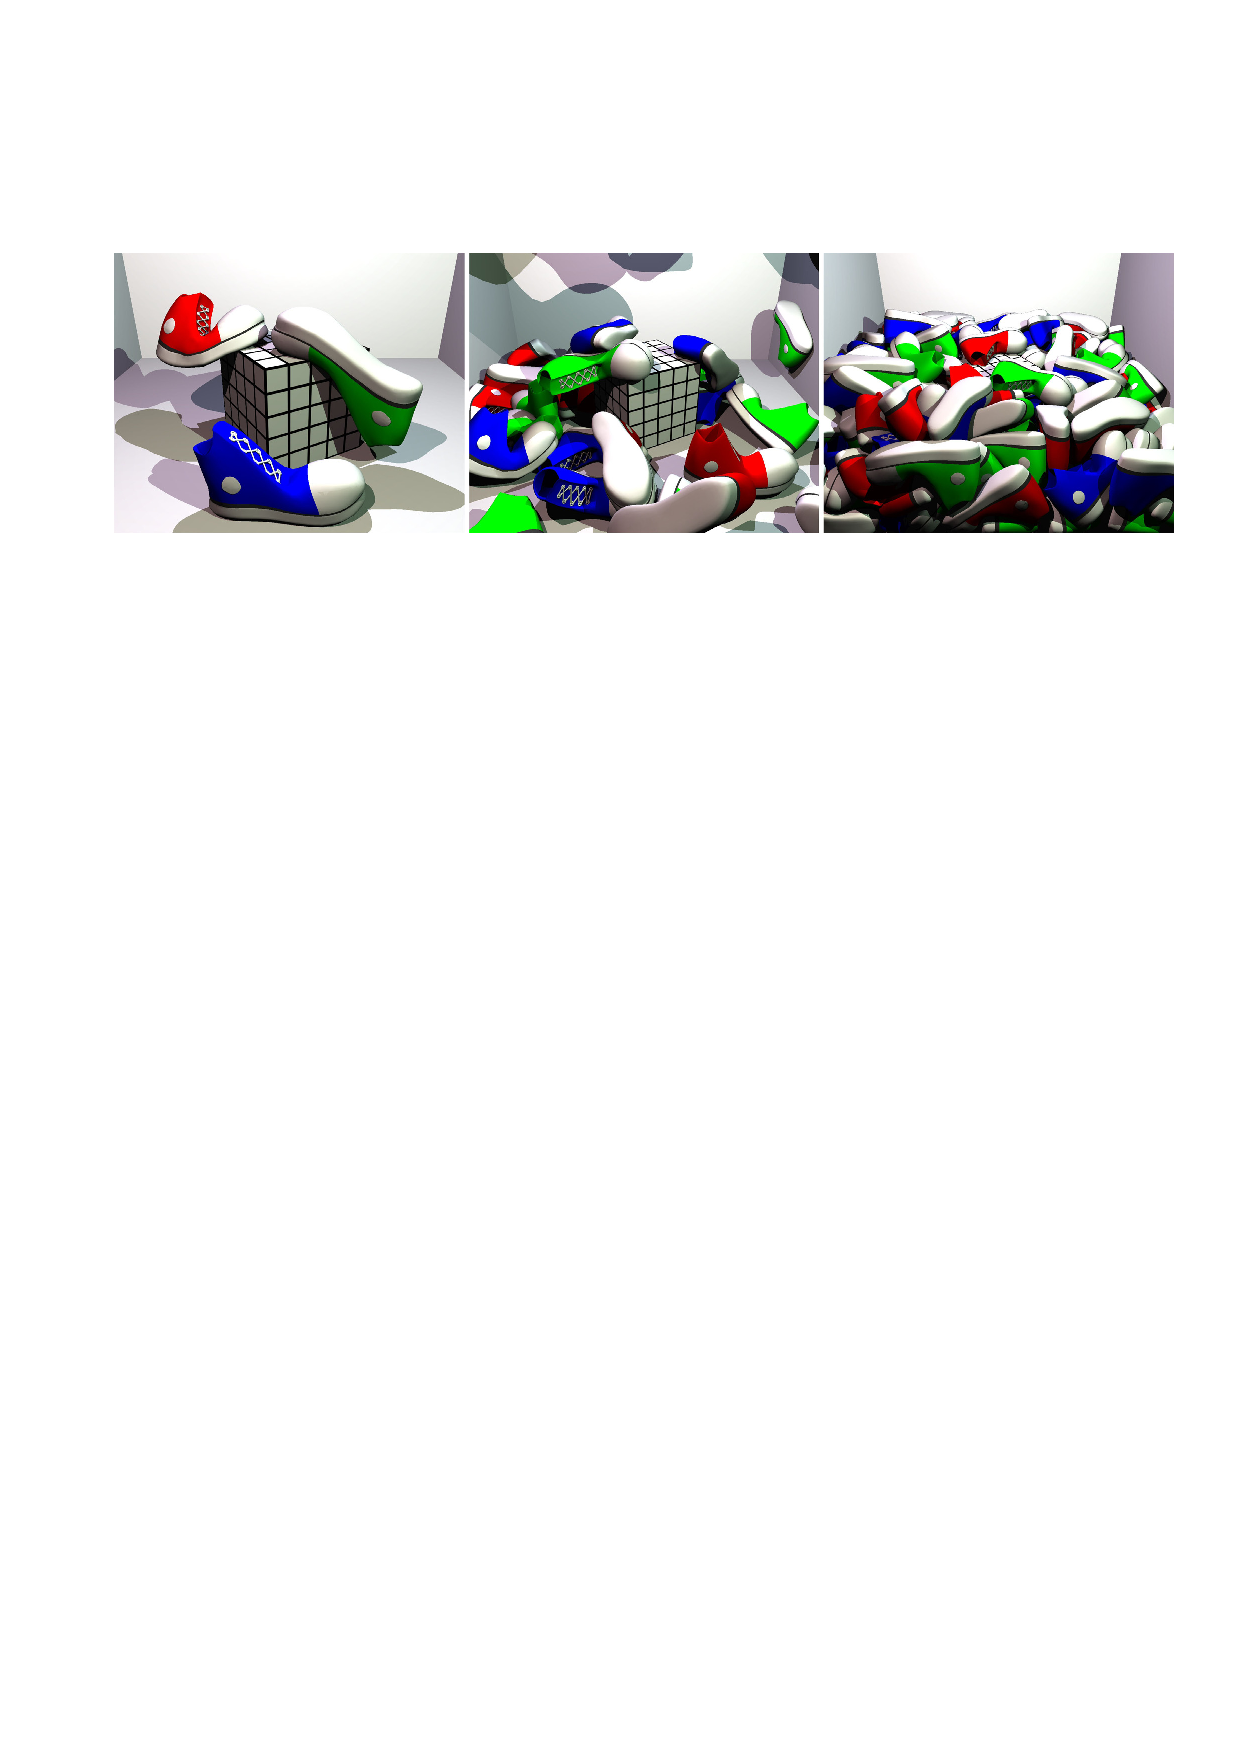
\includegraphics[width=13.9cm]{chapter4/shoes.pdf}
\end{center}
\caption[Shape matching technique]{Shape matching allows to simulate hundreds of deformable objects in real-time.}
\label{chap4:fig-shoes}
\end{figure}

\begin{figure}[h]
\begin{center}
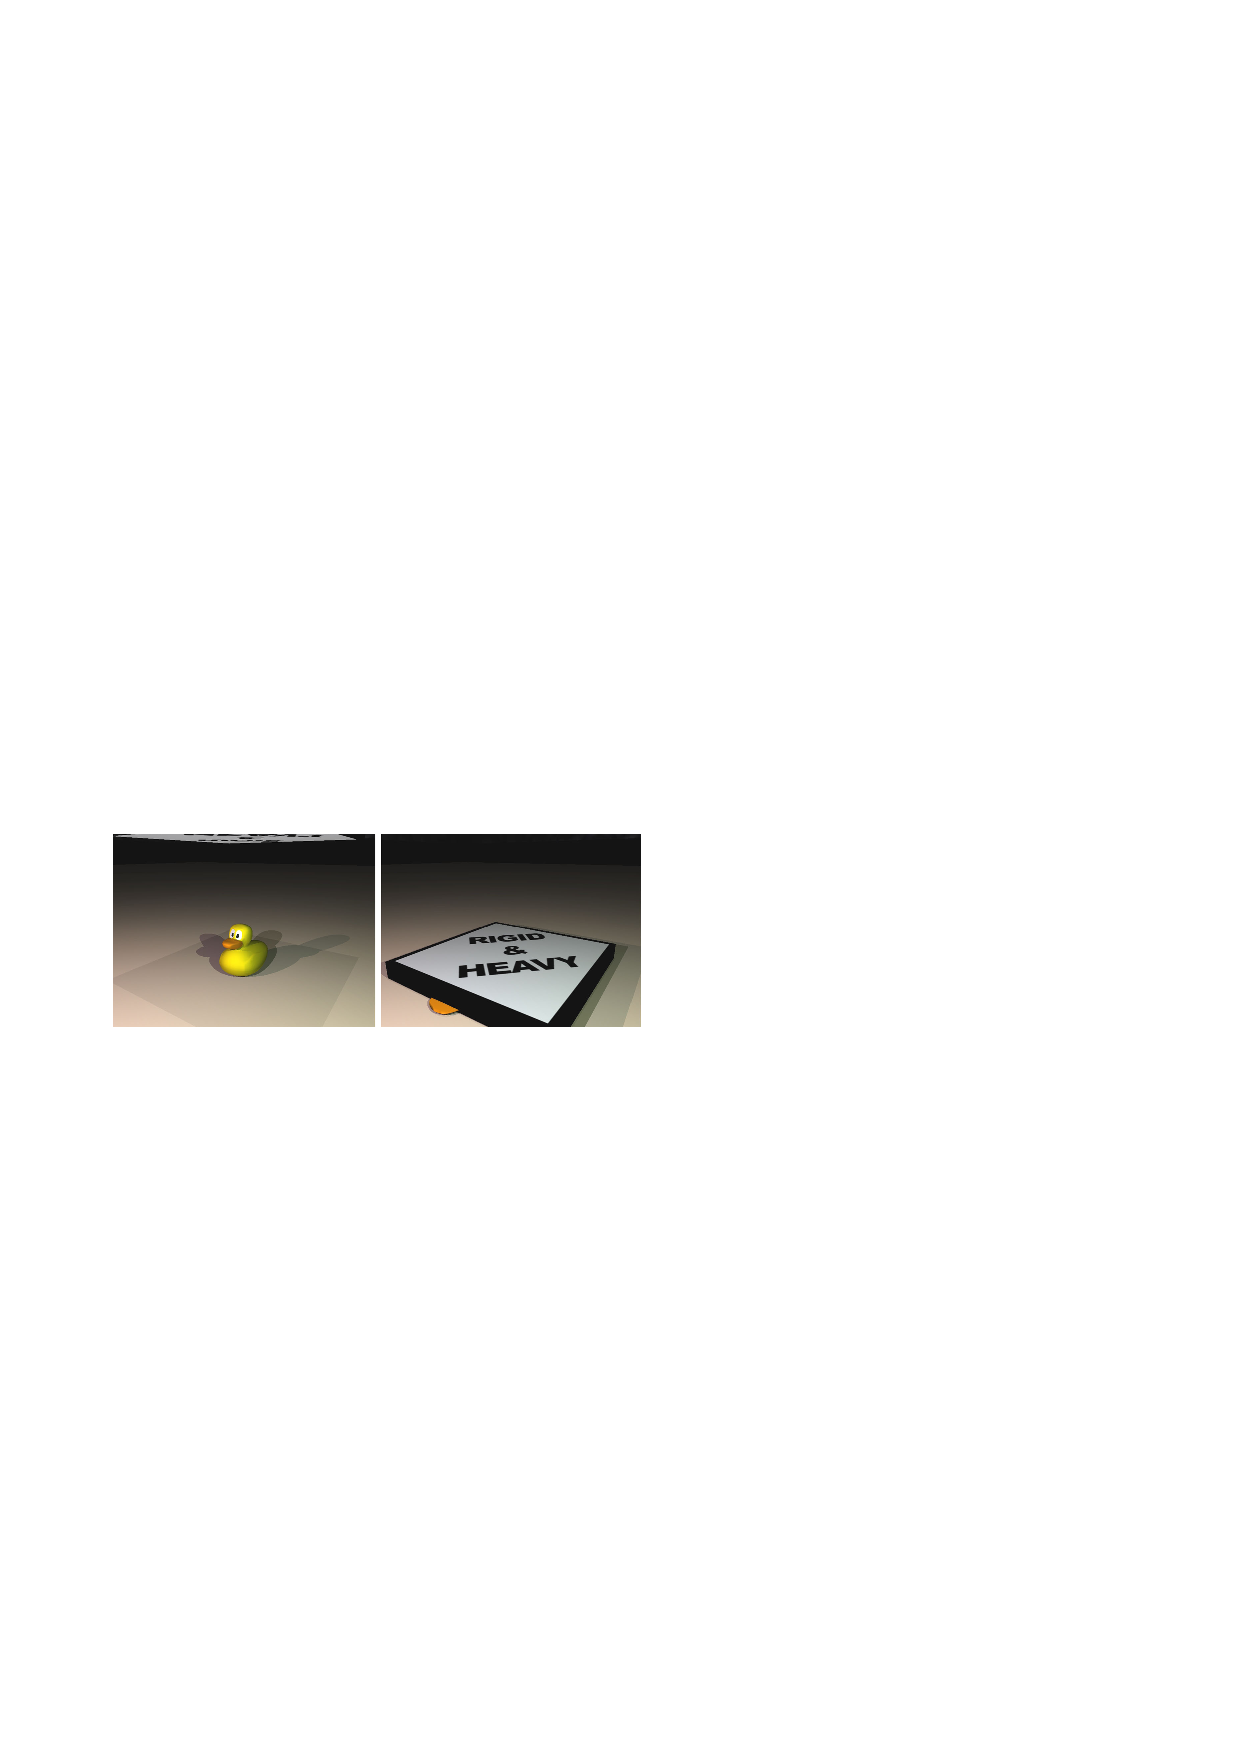
\includegraphics[width=11cm]{chapter4/duck1.pdf} \\
\vspace{0.1cm}
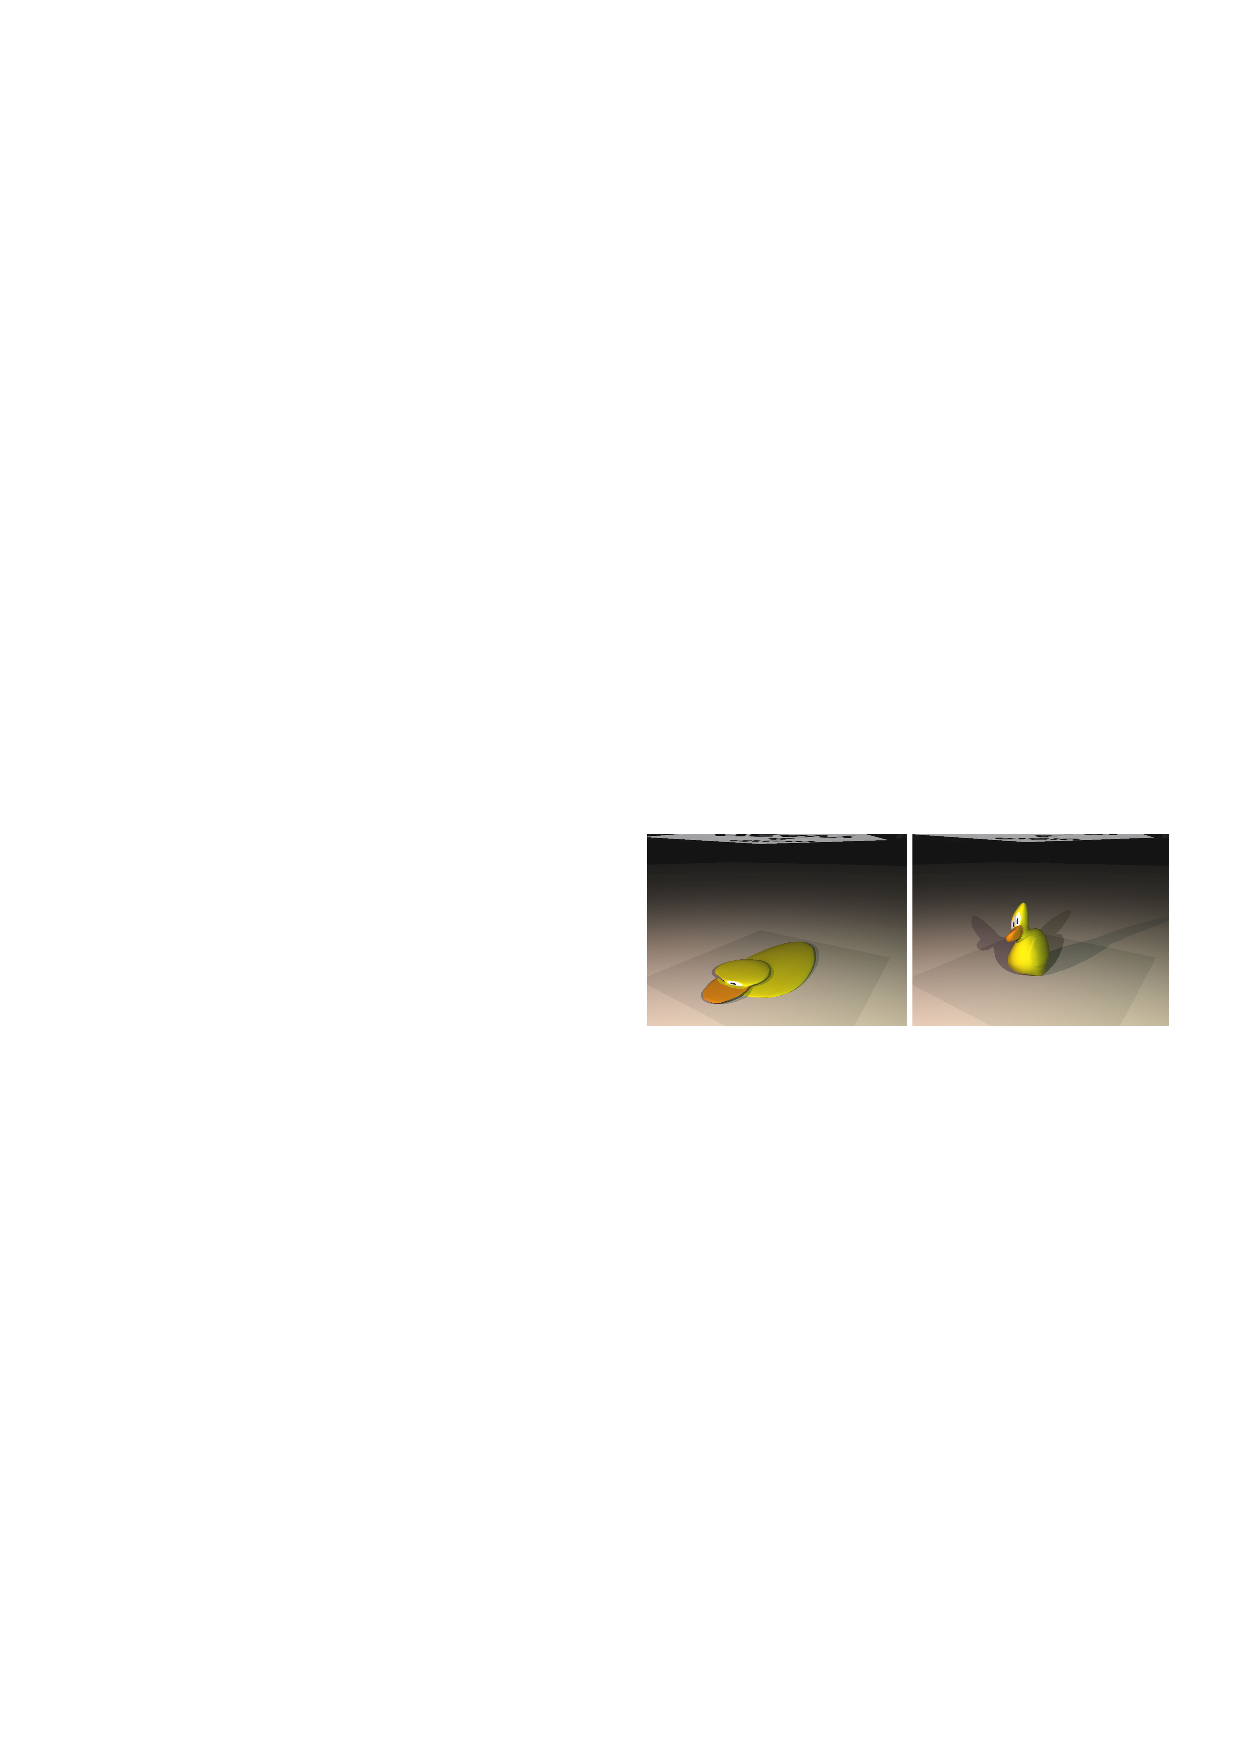
\includegraphics[width=11cm]{chapter4/duck2.pdf}
\end{center}
\caption[Squeezing of a duck using shape matching]{A duck model is squeezed to demonstrate the stability of the shape matching technique. Although the flat shape of the duck is not physically plausible, this example exposes the impressive ability of the approach to recover from highly deformed or inverted configurations.}
\label{chap4:fig-duck}
\end{figure}
	
Later, \cite{Rivers07} extented the technique to regular lattices with embedded geometry. From a surface mesh to be deformed, they start by voxelising the model to construct a lattice of cubic cells containing the mesh. The embedded mesh is then deformed using trilinear interpolation of lattice vertex positions. A particule is placed at each vertex of the lattice and associated with a shape matching region. Their technique of \emph{fast lattice shape matching} allows them to compute per-region transformations in an efficient manner (see \fig{chap4:fig-penguins}).	
%
\begin{figure}[h]
\begin{center}
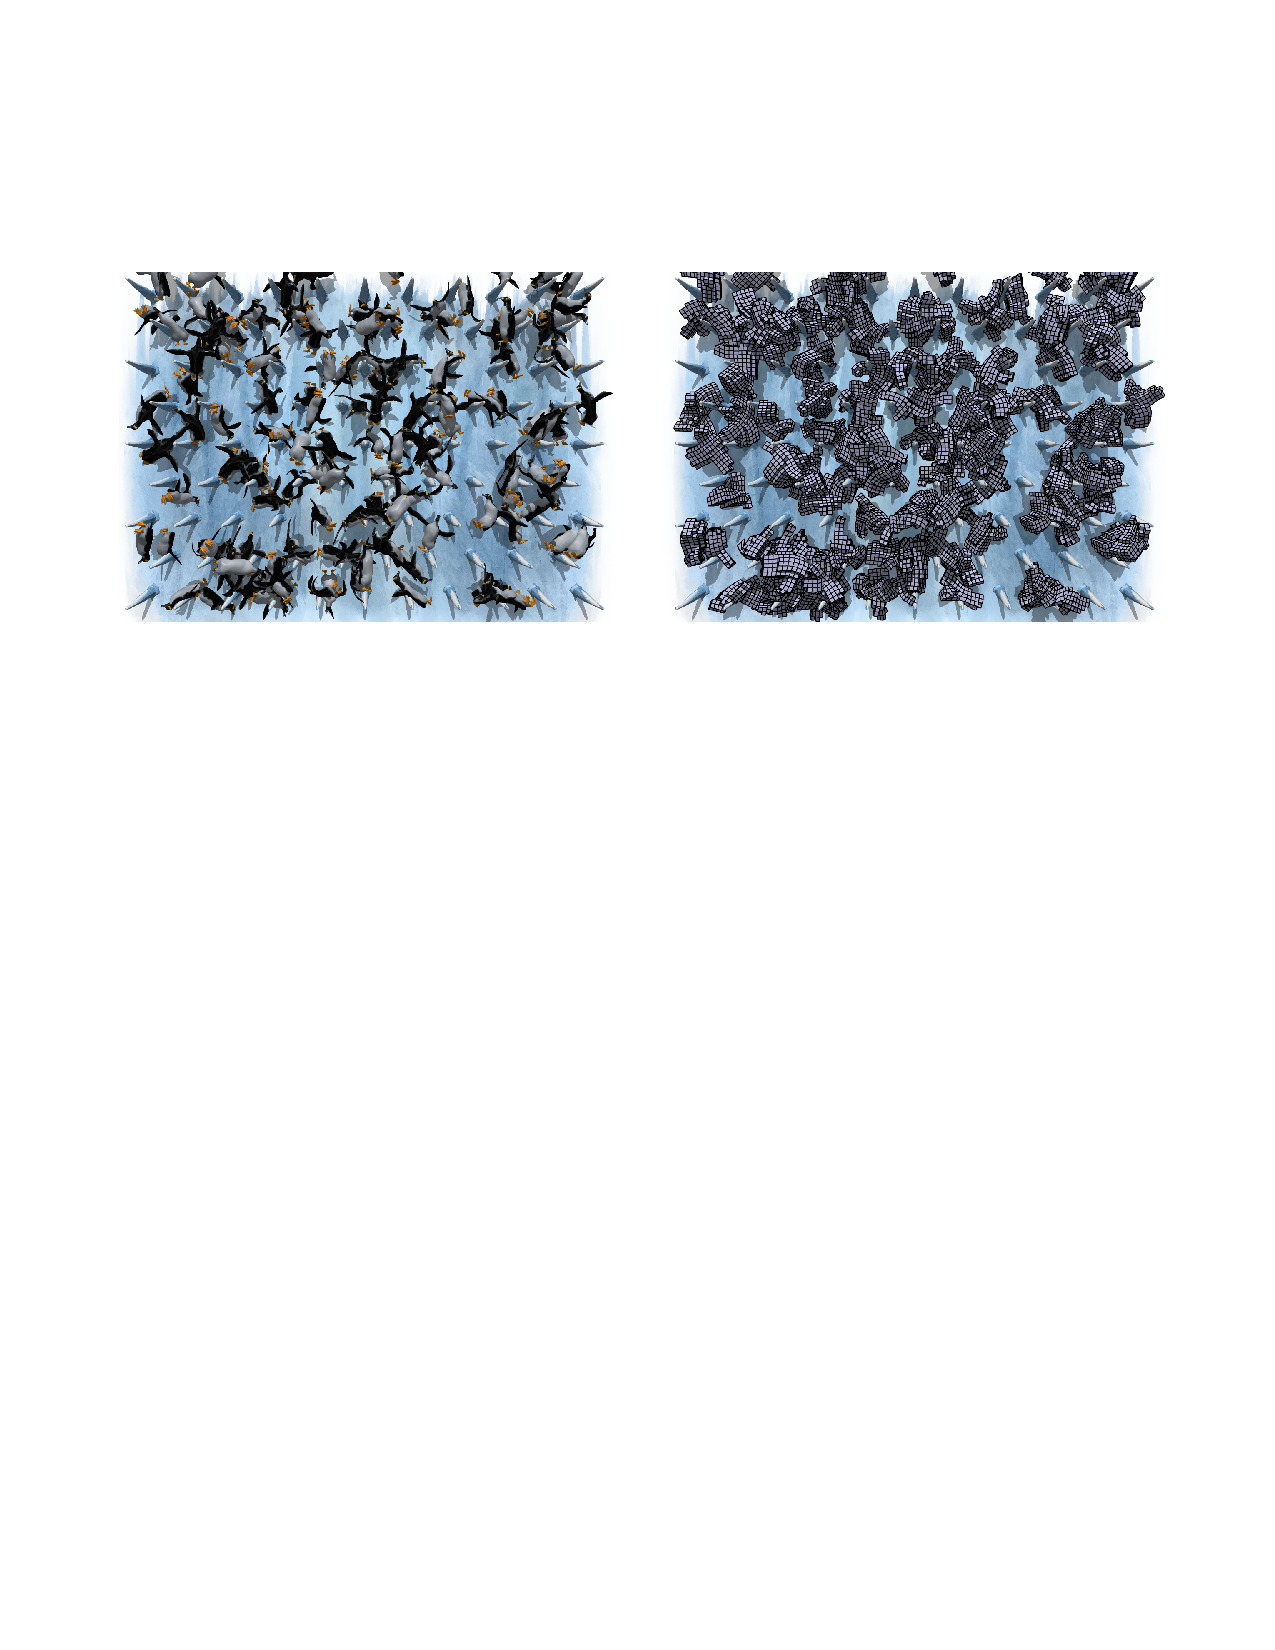
\includegraphics[width=13.9cm]{chapter4/penguins.pdf}
\end{center}
\caption[Penguins animation with fast lattice shape matching]{\textbf{(Left)} $150$ cartoon penguins deforming dynamically using fast lattice shape matching\textbf{(Right)}. Deformed lattices consisting of $150$ particles per penguin ($22\,500$ particles). The penguins can be deformed at $25$ frames per second on a Pentium4 $3.4 \,$GHz.}
\label{chap4:fig-penguins}
\end{figure}

One limitation of fast lattice shape matching is that small features of a geometry yield an explosion of the runtime cost. Indeed, a small surface feature may require fine sampling in order to be deformed independently from non-adjacent material, but this fine sampling must be applied to the whole object. Therefore, \cite{Steinemann08} further improved the technique by allowing dynamic adaptive selection of levels of detail through the use of an octree-based hierarchical sampling. This adaptative sampling is illustrate with \fig{chap4:fig-flowers}. Their technique also handles efficient topological changes.
%
\begin{figure}[h]
\begin{center}
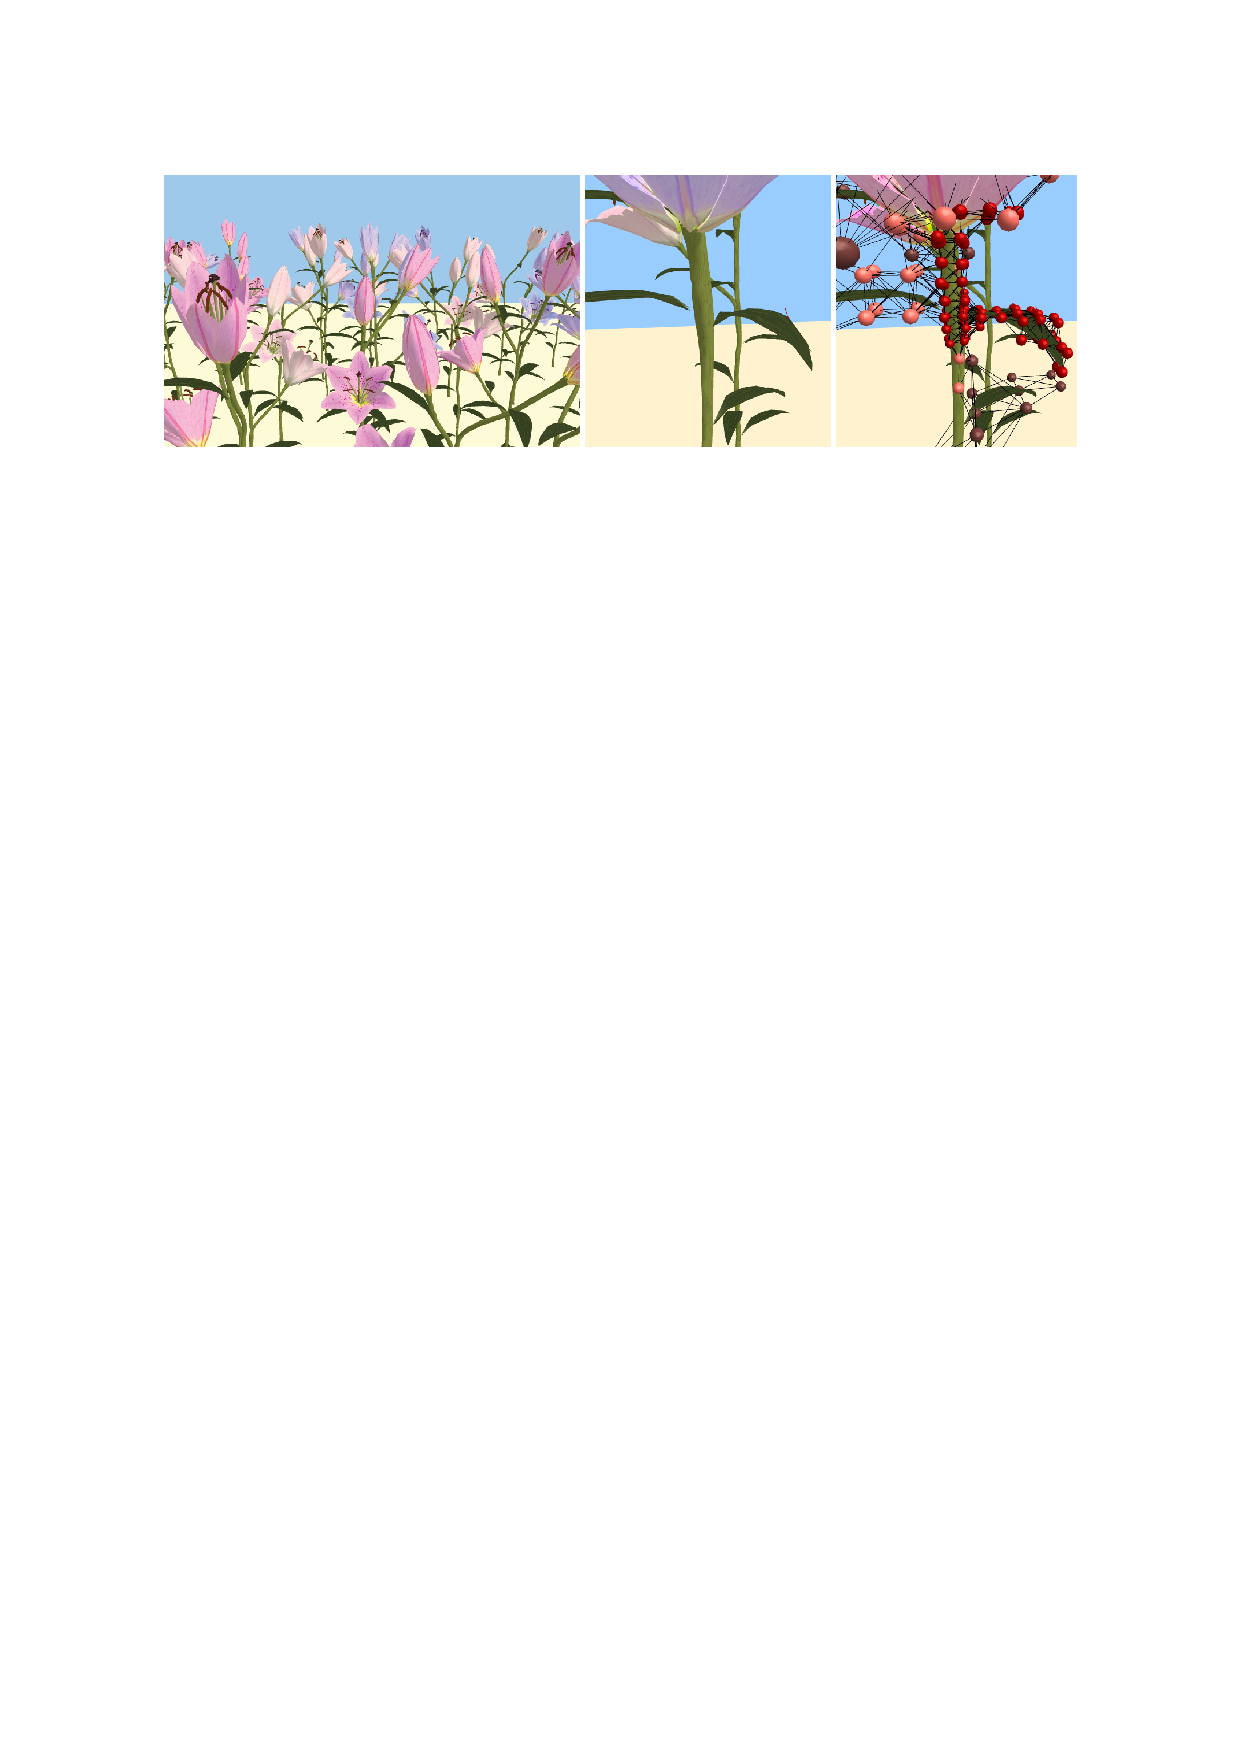
\includegraphics[width=13.9cm]{chapter4/flowers.pdf}
\end{center}
\caption[Flowers in the wind]{Complex scene with $40$ deforming flowers. A coarse sampling is employed when the flowers are moved by the wind, for a total of $5\,680$ nodes in the scene. However, the models are dynamically refined when touched by the user, as shown in the right image.}
\label{chap4:fig-flowers}
\end{figure}	

Although realism is not a crucial feature for game-like environments, other models based on laws of physics were created for other applications.

	
\section{Techniques relying on physics}

	\subsection{3D Chainmail algorithm}
The \emph{3D Chainmail} was introduced by \cite{Gibson97} as a fast algorithm for deforming solid objects. Rather than carrying out complex computations on a low resolution geometry (as opposed to FEM techniques), the main idea is to take advantage of the original data resolution (of a CT scan for instance) but perform simple deformation calculation for each element. In this algorithm, each volume element is linked to its six nearest neighbours. If a link between two nodes is stretched to its limit, displacements are transferred to its neighbouring links. It works in a very similar way to a chain and is illustrated by \fig{chap4:fig-chainmail}. 
%
\begin{figure}[h]
\begin{center}
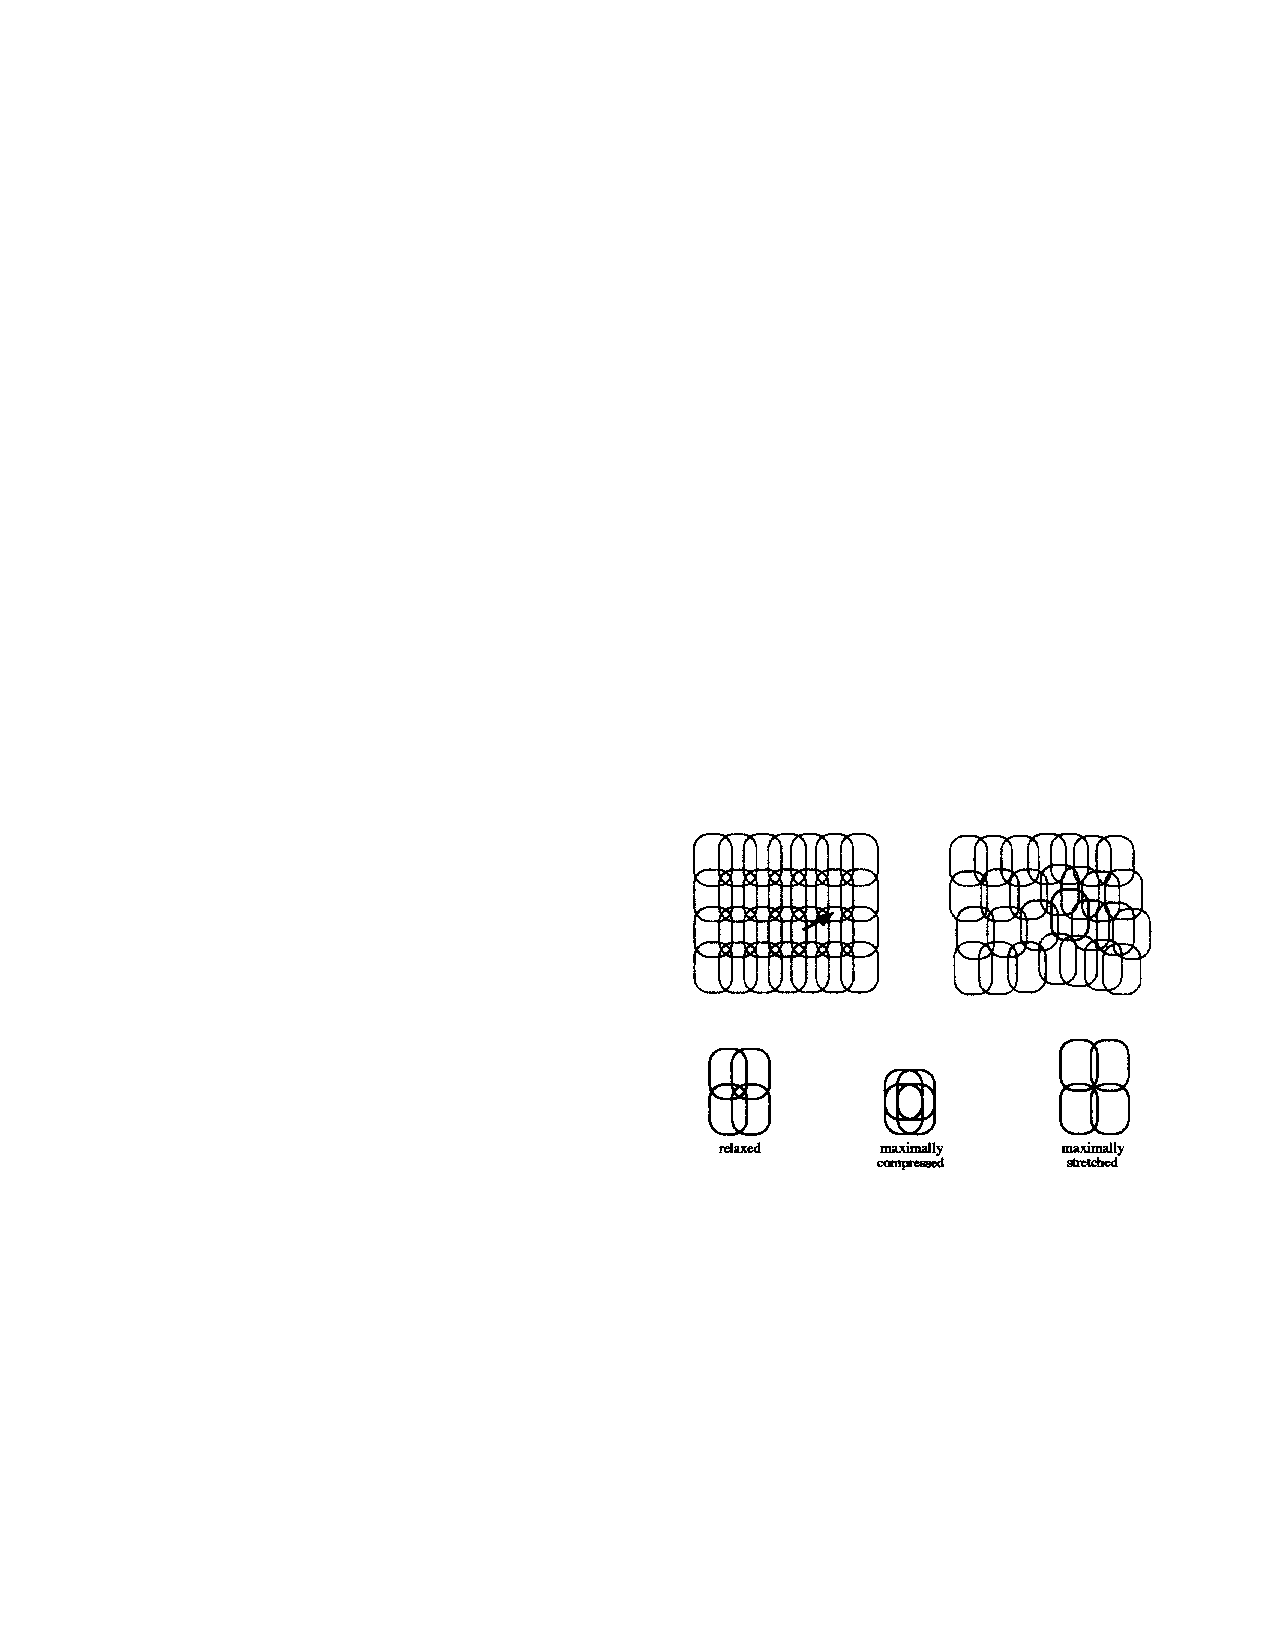
\includegraphics[width=12cm]{chapter4/chainmail.pdf}
\end{center}
\caption[Deformation of a 2D chain]{Deformation of a 2D chain mail when the link indicated by an arrow is moved.}
\label{chap4:fig-chainmail}
\end{figure}	
%
The chain mail algorithm is then followed by an elastic relaxation, which relaxes the shape of the deformed object approximated by the chain mail algorithm. This step consists of minimising an elastic energy measure within the object to insure that the calculated deformation is a minimum energy configuration. 

This method was extented by \cite{Schill98} to integrate inhomogeneous and anisotropic behaviour. This extension of the chain mail algorithm allows the authors to simulate the vitrous humor in the eye during a vitrectomy procedure. However, the main drawback of this algorithm is that it does not model volume preservation, an important characteristic of many tissues in the human body. 


	\subsection{Modal analysis}
\emph{Modal analysis} was first introduced to the graphics community by \cite{Pentland89} as a fast method for approximating deformation. Modal analysis is the process of taking the non-linear description of a system, finding a good linear approximation, and then finding a coordinate system that diagonalises the linear approximation. This process transforms a complicated system of non-linear equations into a simple set of decoupled linear equations that may be individually solved analytically \citep{Hauser03}. Moreover, because each decoupled equation may be solved analytically, stability concerns due to the choice of a time integration procedure are eliminated. The linearised system of equations may be written as:
\begin{equation}
\label{chap4:linearisedEquation}
\mathbf{M} \mathbf{\ddot U} + \mathbf{D} \mathbf{ \dot U} + \mathbf{K} \mathbf{U} = \mathbf{R}.
\end{equation}	
where $ \mathbf{M} $ is the mass matrix, $\mathbf{D}$ is the damping matrix, $ \mathbf{K} $ is the stiffness matrix and $\mathbf{R}$ are the externally applied loads. Modal decomposition refers to the process of diagonalising equation \eqref{chap4:linearisedEquation}. By using Rayleigh damping (see discussion on damping in section \ref{chap3:wordOnMatrices}), \eqref{chap4:linearisedEquation} may be rewritten as:
\begin{equation}
\label{chap4:eqRayleigh}
\mathbf{K} (\mathbf{U} + \alpha_1  \mathbf{ \dot U}) + \mathbf{M} (\alpha_2 \mathbf{ \dot U} + \mathbf{\ddot U})  = \mathbf{R},
\end{equation}	
where $ \alpha_1 $ and $ \alpha_2 $ are the Rayleigh coefficients. We denote $ \mathbf{W} $ the solution to the generalised eigenproblem $ \mathbf{K} \mathbf{x} + \lambda \mathbf{M} \mathbf{x} = 0 $ and $\boldsymbol \Lambda$ the diagonal matrix of eigenvalues, then \eqref{chap4:eqRayleigh} may be expressed as:
\begin{equation}
\boldsymbol \Lambda (\mathbf{Z} + \alpha_1  \mathbf{ \dot Z}) + (\alpha_2 \mathbf{ \dot Z} + \mathbf{\ddot Z})  = \mathbf{G},
\end{equation}
where $ \mathbf{Z} = \mathbf{W}^{-1} \mathbf{U} $ is the vector of modal coordinates and $ \mathbf{G} = \mathbf{W}^T \mathbf{U} $ is the external force vector in the modal coordinate system. Each row of this equation now corresponds to a single scalar differential equation:
\begin{equation}
\ddot z_i + (\alpha_1 \lambda_i +\alpha_2) \dot z_i + \lambda_i z_i = g_i.
\end{equation}
The analytical solutions to each equations are well known and are the following:
\begin{equation}
z_i = c_1 e^{t \omega_i^+} + c_2 e^{t \omega_i^-}
\end{equation}
where $ c_1 $ and $ c_2 $ are complex constants and $ \omega_i $ is the complex frequency given by:
\begin{equation}
\omega_i^{\pm} = \dfrac{-(\alpha_1 \lambda_i + \alpha_2) \pm \sqrt{(\alpha_1 \lambda_i +\alpha_2)^2 - 4 \lambda_i}}{2}.
\end{equation}
The main advantage of modal analysis is the possibility to model only the necessary modes. Indeed if the eigenvalue $ \lambda_i $ associated with a particular mode is large, then the force required to cause a discernible displacement of that mode will also be large. Similarly, some displacements may be too small to be detected. Removing those modes from the computation will not change the appearance of the resulting simulation while substantially reducing the computational cost. 

\cite{James02} went even further by using graphics hardware to reduce CPU costs to a minimum. In particular, they use modal analysis to model human skin and secondary tissues in a laparascopic surgical simulation to allow the CPU to focus on more complex tissue models and user contact interactions (see \fig{chap4:fig-modalAnalysisLaparo}). The technique is fairly efficient as it allows precomputations of the vibration modes. 
%
\begin{figure}[h]
\begin{center}
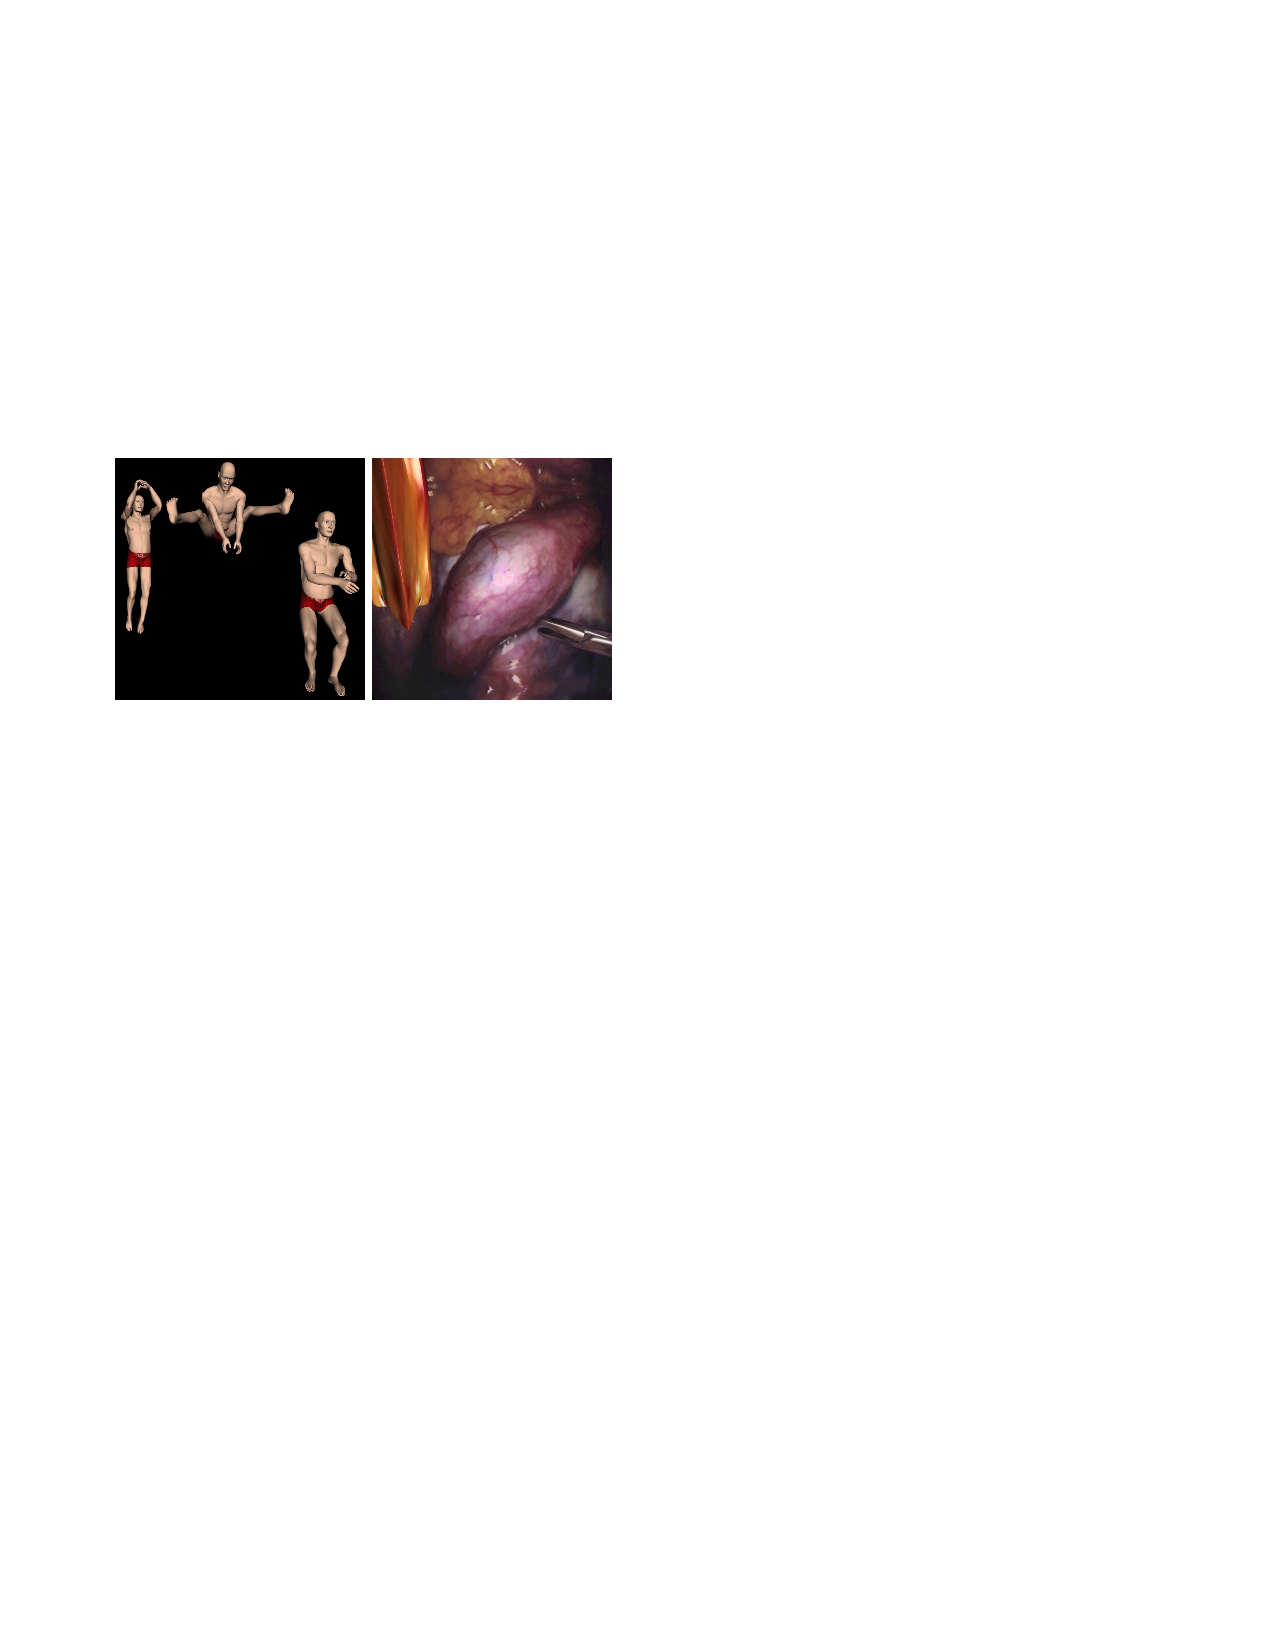
\includegraphics[width=13cm]{chapter4/modalAnalysisLaparo.pdf}
\end{center}
\caption[Applications of modal analysis]{(\textbf{Left}) A jumping motion that leads to significant thigh and belly vibrations of human skin when rendered with modal analysis. (\textbf{Right}) The same hardware accelerated technique is applied to secondary tissues in a laparoscopic simulation to ease the CPU of computations. } 
\label{chap4:fig-modalAnalysisLaparo}
\end{figure}	

Although modal analysis significantly accelerates the simulation, it generates noticeable artifacts when applied to large deformations due to the step of linearisation. It can produce unnatural results with deformations of large amplitude. \cite{Choi05} proposed to overcome this limitation by taking the rotational component of the deformation into account at each node. \cite{Barbic05} make use of modal analysis to build a deformation basis from modal derivatives. It allows them to simulate large deformations of solid objects with non-linear material. 


	\subsection{Mass-spring model}	\label{chap4:massSprings}
A classic technique for modelling a deformable object is the mass-spring system. In this method, the geometry is described by a network of masses connected together by springs. The force $ F $ exerted onto each mass by the spring may be computed with:
\begin{equation}
\label{chap4:massSpring1}
F_{\text{spring}} = - k x,
\end{equation}
where $ k $ is the spring stiffness constant, $ x $ represents the stretch of the spring from its rest position. From our experience, we know that a mass attached to a single spring has a tendency to oscillate. If no appropriate measure is taken, a network of springs will a forciori oscillate as well. To prevent the system from oscillating, a damper is also added between each couple of masses. The force created by the damper acts to reduce the velocity and may be expressed as:
\begin{equation}
\label{chap4:massSpring2}
F_{\text{damper}} = - d v
\end{equation}
where $ d $ is the damping constant and $ v $ the derivative of $ x $ with respect to time. The damper added between each couple of masses allows to model friction and reduce the amplitude of the oscillations. Applying Newton's second law $ \sum \mathbf{F} = m \mathbf{a} $ yields the standard differential equation for a mass-spring system:
\begin{equation}
\label{chap4:massSpring3}
m \ddot x = - d \dot x - k x.
\end{equation}
For complex systems with more than one spring attached to each mass, the right-hand side of the equation \eqref{chap4:massSpring3} becomes more complex as it needs to be repeated and adjusted for each spring. The easiest way to solve a complex mass-spring system iteratively, is to first calculate the total force currently acting on each mass by summing all forces currently exerted by all springs attached to this mass (using \eqref{chap4:massSpring1} and \eqref{chap4:massSpring2}). Dividing the total force by the mass gives the current acceleration of each mass (by \eqref{chap4:massSpring3}). This equation must be numerically solved for each mass, either by explicit or implicit methods. A discussion of integration methods for mass-spring models can be found in \cite{Shinya05}. 

Mass-spring systems have been extensively used and are still very popular. And this is not surprising because they are easy to implement and computationally efficient. Of course, they have drawbacks. But as we will see shortly, various recent works attempt to circumvent them. One limitation often mentioned is the difficulty to derive spring stiffnesses from elastic properties (Young's modulus and Poisson's ratio). To overcome this deficiency, \cite{Lloyd07} mention two ways of obtaining the parameters of a mass-spring model. The first one consists in varying the parameters until the behaviour of the system is similar to the one obtained through the experiments or the one obtained with the Finite Element Method \citep{Bianchi04}. The second way consists in establishing an analytical reasoning for calculating the constants of the mass-spring model. For instance, starting from the definition of Young's modulus, Poisson's ration, shear and bulk modulus, \cite{Baudet07} apply simple tests to their mass-spring model to find the most appropriate stiffnesses. \cite{Lloyd07} proposes a linearisation of the mass-spring equations with the aim of equating the linearised stiffness matrix to the stiffness matrix of a linear finite element method. By following the same method, \cite{SanVicente09} derived a mass-spring model equivalent to a linear finite element model for maxillofacial surgery simulation. 

Because they do not derive from the equations of continuum mechanics, mass-spring models have a limited capacity to model the various aspects of a material like anisotropy, viscoelasticity etc. Even worse, according to \cite{Bourguignon00}, if all springs are set to the same stiffness, the mesh geometry may generate undesired anisotropy as shown in \fig{chap4:fig-undesiredAnisotropy}. However, some works tried to take advantage of this feature by giving directions of interest to their model by specifically designing the mesh to align springs on specific directions. For instance, it was used by \cite{Miller88} to animate the motion of snakes and worms. It was also used by \cite{Ng-Thow-Hing97} in their muscle model where some of the springs were aligned with the muscle fibers and more recently by \cite{Magjarevic09} for modelling the mechanical behavior of the myocardial tissue. More details on controlling anisotropy in mass-spring systems may be found in \cite{Bourguignon00}. 
%
\begin{figure}[h]
\begin{center}
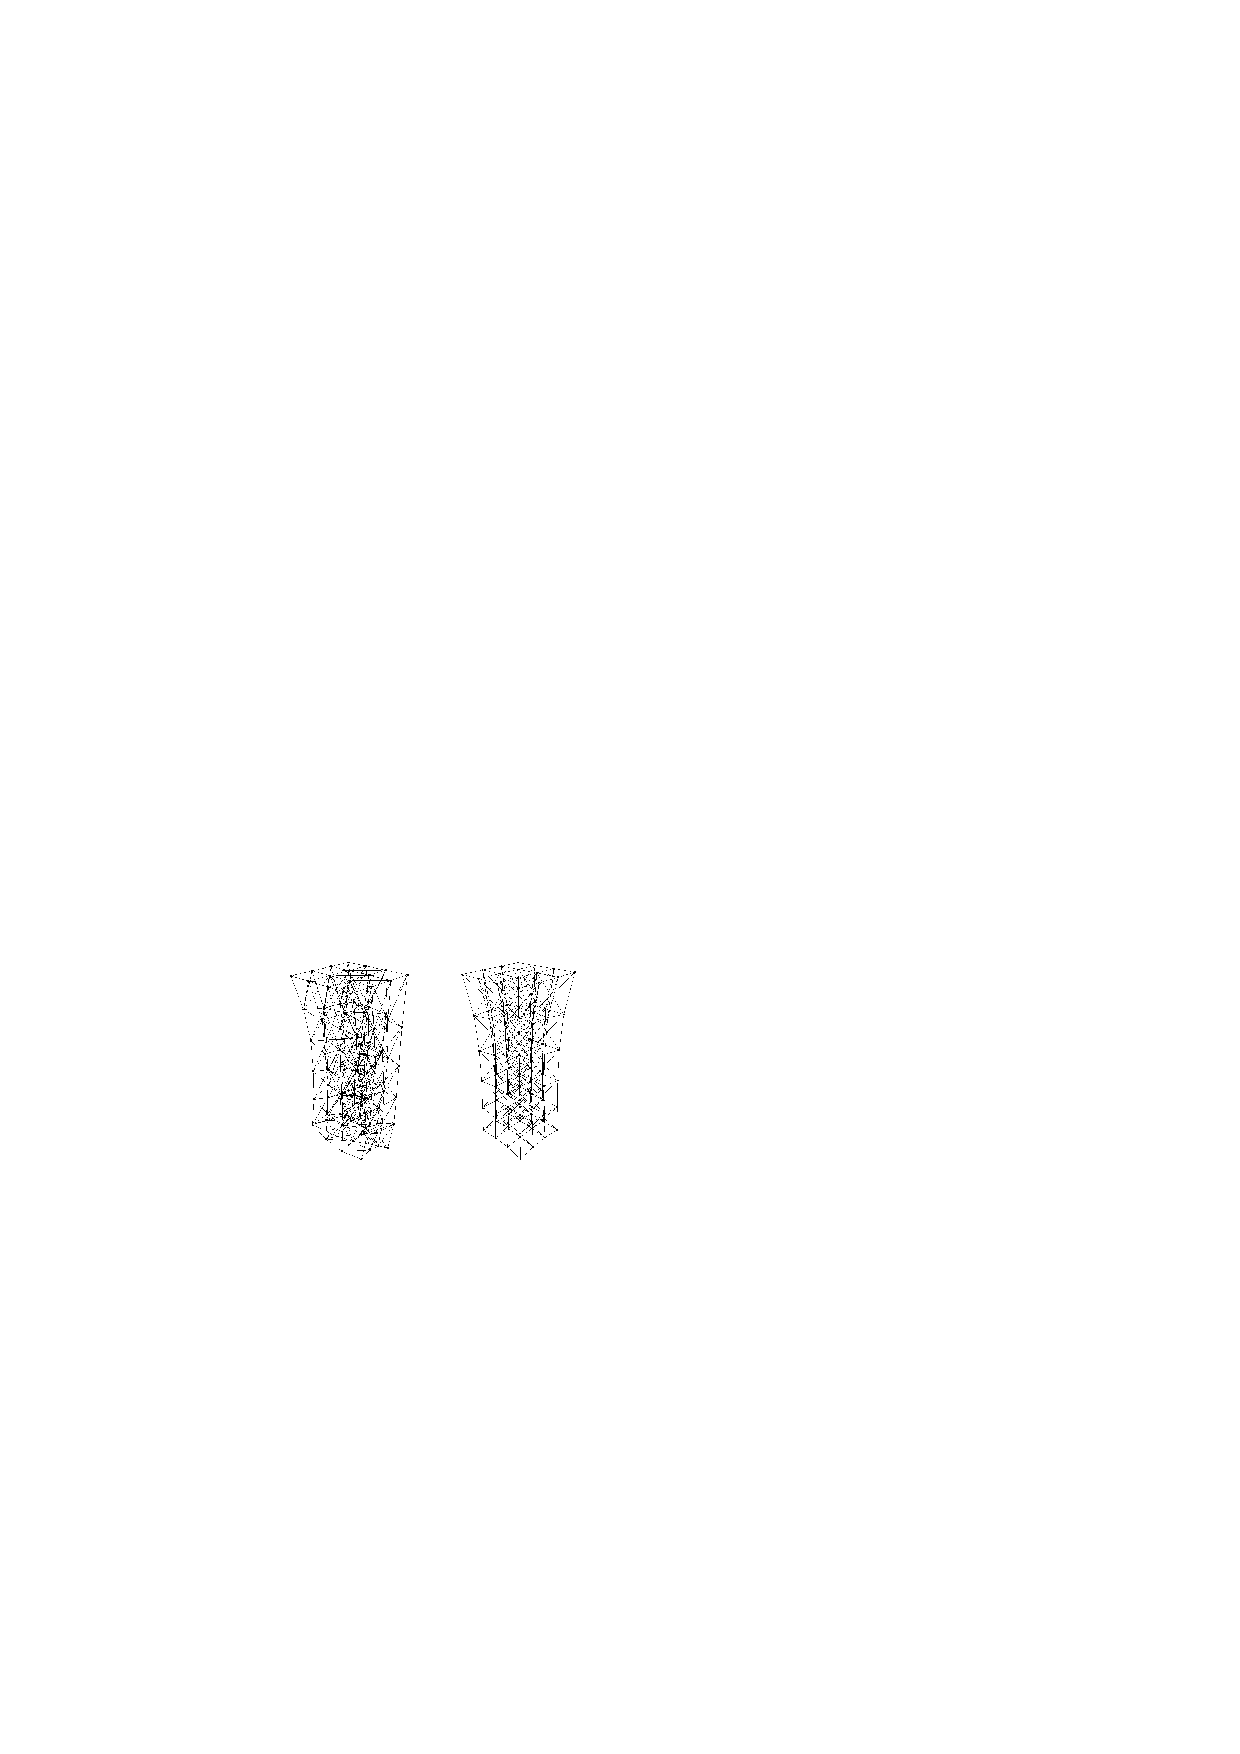
\includegraphics[width=8cm]{chapter4/undesiredAnisotropy.pdf}
\end{center}
\caption[Undesired anisotropy with mass-spring models]{The two meshes are undergoing a downward pull at their bottom. While the tetrahedral mass-spring system \textbf{(left)} shows signs of anisotropy, the hexahedral mesh \textbf{(right)} with springs aligned along the gravity does not.} 
\label{chap4:fig-undesiredAnisotropy}
\end{figure}	

A mass-spring model may also be enhanced to feature viscoelasticity. Indeed, \cite{Stiles72} proposed a viscoelastic mass-spring system to test hypotheses on the mechanical response of muscles. Much more recently, \cite{Tamura05} introduced a method to simulate viscoelastic material using a mass-spring system. They use a large number of particules to create a randomly connected mesh to mimic the structure of polymeric materials and hence their viscoelascity characteristics. \cite{Basafa10} went even further and extended a mass-spring system to simulate non-linear viscoelastic deformations of soft tissue for laparoscopic surgery. They tune their parameters by a simple optimisation procedure to fit the mechanical response obtained on a set of experimental data. 

\cite{Terzopoulos91} even designed a mass-spring system that experience transitions from solid to liquid. Nodes are connected by springs in a hexahedral lattice and each of them has an associated temperature. Spring stiffnesses decreased with the increase in temperature. The diffusion of heat through the material is computed by using a discretised form of the heat equation. When the melting point is reached, the stiffness is set to zero and the node is detached from this particular spring. Once a node is freed from all his neighbouring springs, it becomes an independent glop of fluid and its behaviour is then modelled using a discrete fluid model. 

\bigskip

Early 2000s, the rapid increase in the performance of graphics hardware, coupled with recent improvements in its programmability, have made graphics hardware a compelling platform for computationally demanding tasks in a wide variety of application domains. Researchers and developers have become interested in harnessing this power for general-purpose computing, an effort known collectively as GPGPU (for General-Purpose computing on Graphics Processing Units). A survey of GPGPU algorithms and techniques was written by \cite{Owens07}.

\cite{Mosegaard05a,Mosegaard05b} were probably the first to implement a mass-spring model on GPU in medical simulation. For the first time, the whole simulation of was performed on the GPU (physics, interaction and visualisation) and they used their framework in a congenital cardiac surgery simulation. They compared two implementations: the first one explicitly defined the connectivity between springs using a connectivity texture while the second one determines implicitly determines at runtime that springs are connected when they are neighbours. They were able to compute 188 iterations per second on a $42\,745$ particule model of a pig heart. Depending on the size of the model and the type of implementation, the authors achieved speed-ups between 10 and 30 $ \times $ over their CPU implementation. 

Taking advantage of the GPU to reach a substantial speed-up is usually not straightforward. One must understand the limitations inherent in its design and devise algorithms accordingly. With this idea in mind, \cite{Sorensen06} reviewed the most important concepts and data structures required to realise two popular deformable models on the GPU: the spring-mass model and the finite element model. 

\TODO{Other GPU-based mass-spring implementations?}

If mass-spring systems are quite versatile and easy to implement, the most complete mathematical formalism available to describe the mechanical behaviour of a solid is provided by continuum mechanics. Consequently, it feels natural to derive computational models from the equations of continuum mechanics and a few techniques based on these equations will now be introduced. 
	
		
\section{Techniques based on continuum mechanics}	

	\subsection{The finite element method}
The finite element method brings accuracy a step further. The method will not be explained here since it was already discussed with great details in chapter~\ref{chap3}. This is the method of first choice for modelling deformable objects with precision as it is directly derived from the most complete theory available for describing the mechanical response of a continuum. Different kind of analysis may be carried out with the finite element method. As seen in section~\ref{chap3:derivationEquations}, an analysis may be either static (that is, the transient response is ignored) or dynamic (more general). In all analyses, the deformation of the body at a point is described by some measure of strain. If this measure is chosen to be linear (see section~\ref{chap2:infinitesimalStrainTensor} for details), the analysis is said to be \emph{geometrically} linear. In general, we consider this assumption to be valid for strain less than $ 10 \,$\%. In contrast, geometrically non-linear analyses make use of a non-linear strain tensor to measure the deformation and thus may handle large deformations. Another characteristic of an analysis is whether the relationship between strain and stress (the constitutive model) is assumed to be linear or non-linear. The analysis is qualified as \emph{materially} linear or non-linear, respectively. 

Because of its complexity, the finite element method is substantially more computationally expensive than the ones introduced so far. And this has been a problem in computer graphics and interactive simulation for many years. So researchers came up with simplifying assumptions and ideas to make the computations more efficient. Over time, with the increase in computational power, the simplifications were progressively relaxed and the observed tendency for real-time simulation is now towards more and more complete finite element methods. In this section, we will describe this evolution in the use of finite element methods for interactive simulation. 

\bigskip

The use of the finite element method in computer graphics was pioneered by \cite{Terzopoulos87} for simulations of elastic deformations. They derived a geometrically non-linear strain tensor from differential geometry theory. Obviously, the computations were not carried out in real-time but this technique allows \citeauthor{Terzopoulos87} to calculate the interaction between solid and deformable models in a physically realistic manner (see \fig{chap4:fig-ball}).
 %
\begin{figure}[h]
\begin{center}
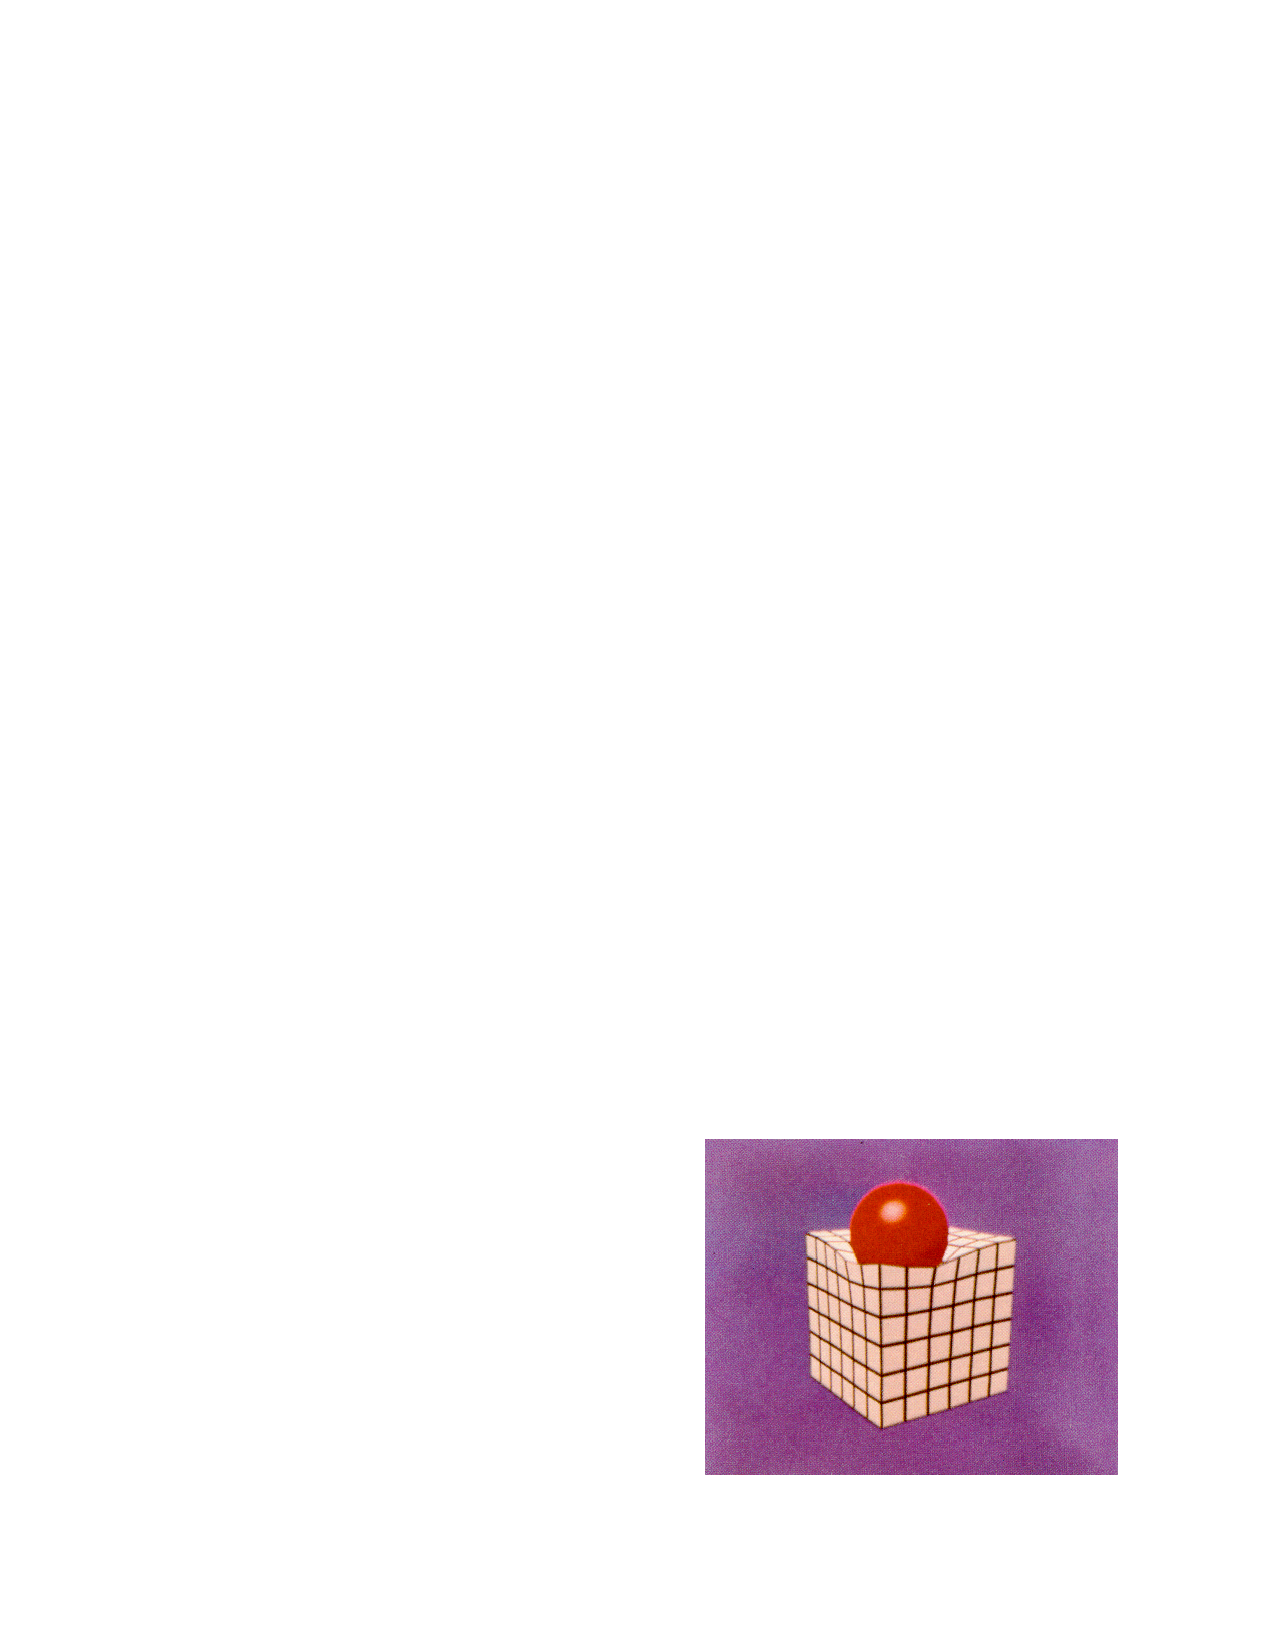
\includegraphics[width=7cm]{chapter4/ball.pdf}
\end{center}
\caption[Ball on a deformable model]{A ball resting on a supporting elastic solid as computed by \citeauthor{Terzopoulos87}.} 
\label{chap4:fig-ball}
\end{figure}	
In order to speed up the computations, linear strain measures started to be used (see section~\ref{chap2:infinitesimalStrainTensor}). For instance, \cite{Gourret89} make use of a linear finite element method to model the deformation of grasped objects. The equations are however solved in static for simplicity. An approach to solve the system of equations in dynamic in a reasonable amount of time is to decrease the number of elements. This reduction must be compensated by the use of high-order elements, that is the degree of the shape functions used in the interpolation of the solution is higher to maintain the overall accuracy. This approach was applied to an elaborate model of a muscle by \cite{Chen92} and to modelling skin in a simulator of plastic surgery by \cite{Pieper92} where they both use 20-node brick elements. Yet, finite element modelling remained very computationally expensive and the interactivity required for medical simulators was still to be reached. 

In 1996, \citeauthor{Bro-Nielsen96} developed a real-time finite element method formulation by introducing three improvements. The first one is to compress the stiffness matrix of the volumetric system into a matrix with the same complexity as a surface model of the same object. This technique is called \emph{condensation}. The deformation is solved only at surface points while still taking the volumetric nature of the object into account. The second improvement concerns the fact that they explicitly precompute the inverse of the stiffness matrix and use matrix vector multiplication with this matrix to achieve a low calculation time. Finally, they exploit the sparse structure of the force vector. They showed the efficiency of their method by modelling a leg with 700 nodes at 20 frames per second. 

Later, \cite{James99} had another idea to improve the speed of the computation. They based their model on boundary integrals and the \emph{boundary element method}, used for the first time in computer graphics. The method consists of calculating only boundary displacements and forces. Unfortunately, the authors do not provide the performance of their framework.

\cite{Cotin99} took advantage of the superposition principle which applies to linear problems. Their idea was to approximate the deformation of a solid object with a linear combination of pre-computed states. In addition, they enhanced the formulation by adding a non-linear radial component. This method was applied to compute the deformation of liver in a hepatic surgery simulator. Their approach substantially improved the computational time for a finite element model as it allowed them to compute the positions and the forces of a $1\,500$ node liver at $300\,$Hz. An important drawback emphasised by the authors themselves is the impossibility to simulate tissue cutting. Indeed, the large precomputations associated with this method are dependent of the geometry of the mesh and therefore cannot be updated in real-time. 

\bigskip

Besides real-time computation of soft tissue, another major concern for medical simulators is the ability to cutting through soft tissue models. \cite{Mor00} proposed a technique to generate a minimal set of new elements to replace intersected tetrahedra along the path formed by the cut. The method do not wait for the cut to be completed for splitting an element, instead, a minimal subdivision of a partially cute tetrahedron is generated. The authors used a very small time step to insure the stability of the soft tissue model and their simulations were not real-time. In addition, their method can create very small elements and the model can become unstable. This occurs because the stiffness matrices for the small elements are quite large, and even small displacements can generate very large forces. 

\cite{Cotin00} proposed a hybrid model allowing real-time cutting. They combined a quasi-static precomputed model, which is very efficient but does not allow topology changes, with a tensor-mass model which requires more computation but authorises cutting. The key idea is to separate a same structure into two parts: one susceptible to be cut during the surgery procedure and one that will not be submitted to any topological change. While the former will be simulated with the tensor-mass model, the deformation of the latter will be computed using the precomputed model. Since both linearly elastic models follow the same physical law, the combination of these two models should behave exactly as a global, linearly elastic model. To achieve this goal, \citeauthor{Cotin00} describe how to impose the additional boundary conditions at the connection nodes for the global model to be consistent in terms of forces and displacements. The efficiency of this hybrid model was demonstrated by simulating an hepatectomy (removing of one of the eight anatomical segments of the liver). They reported the simulation (allowing deformation and cutting) of a mesh with more than $ 8\,000 $ tetrahedra in real-time (see \fig{chap4:fig-hybridModel}).
%
\begin{figure}[h]
\begin{center}
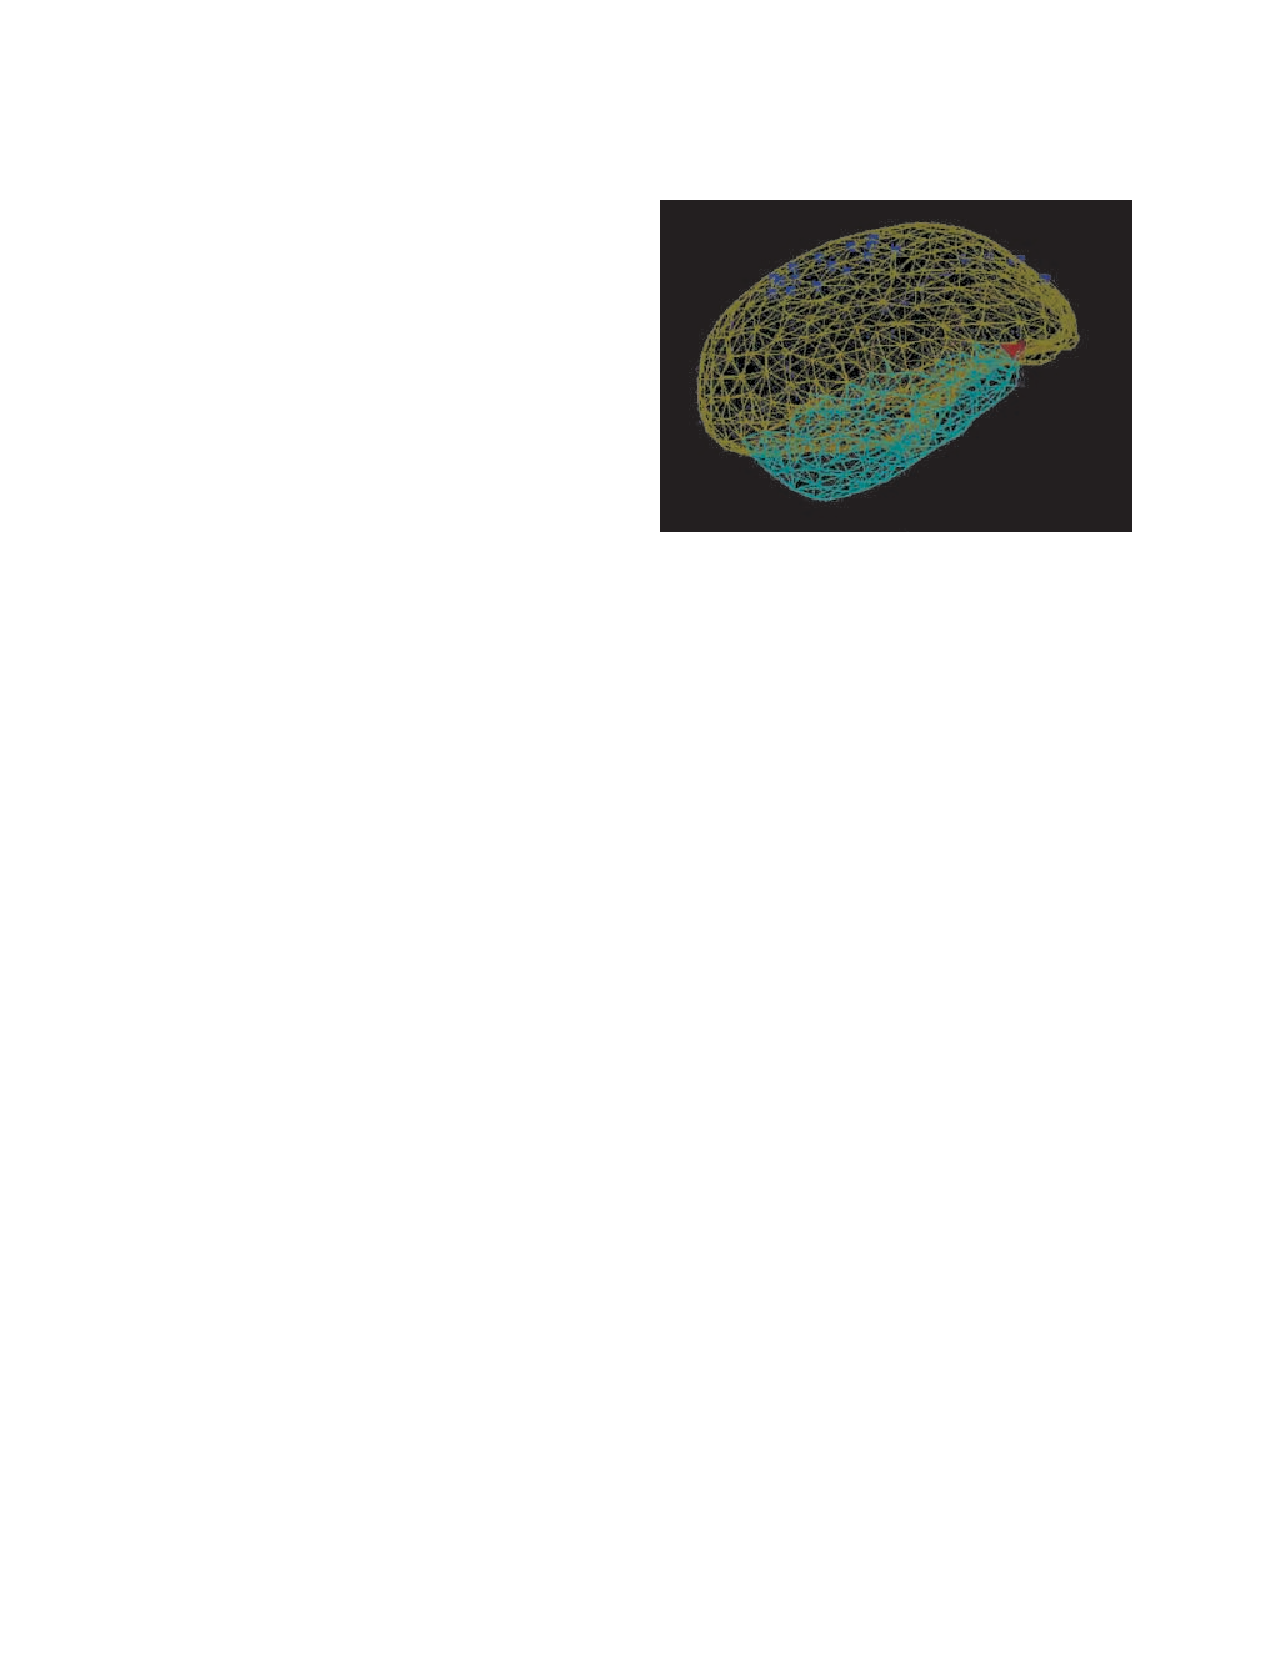
\includegraphics[height=4.5cm]{chapter4/hybrid1.pdf}
\hspace{0.2cm}
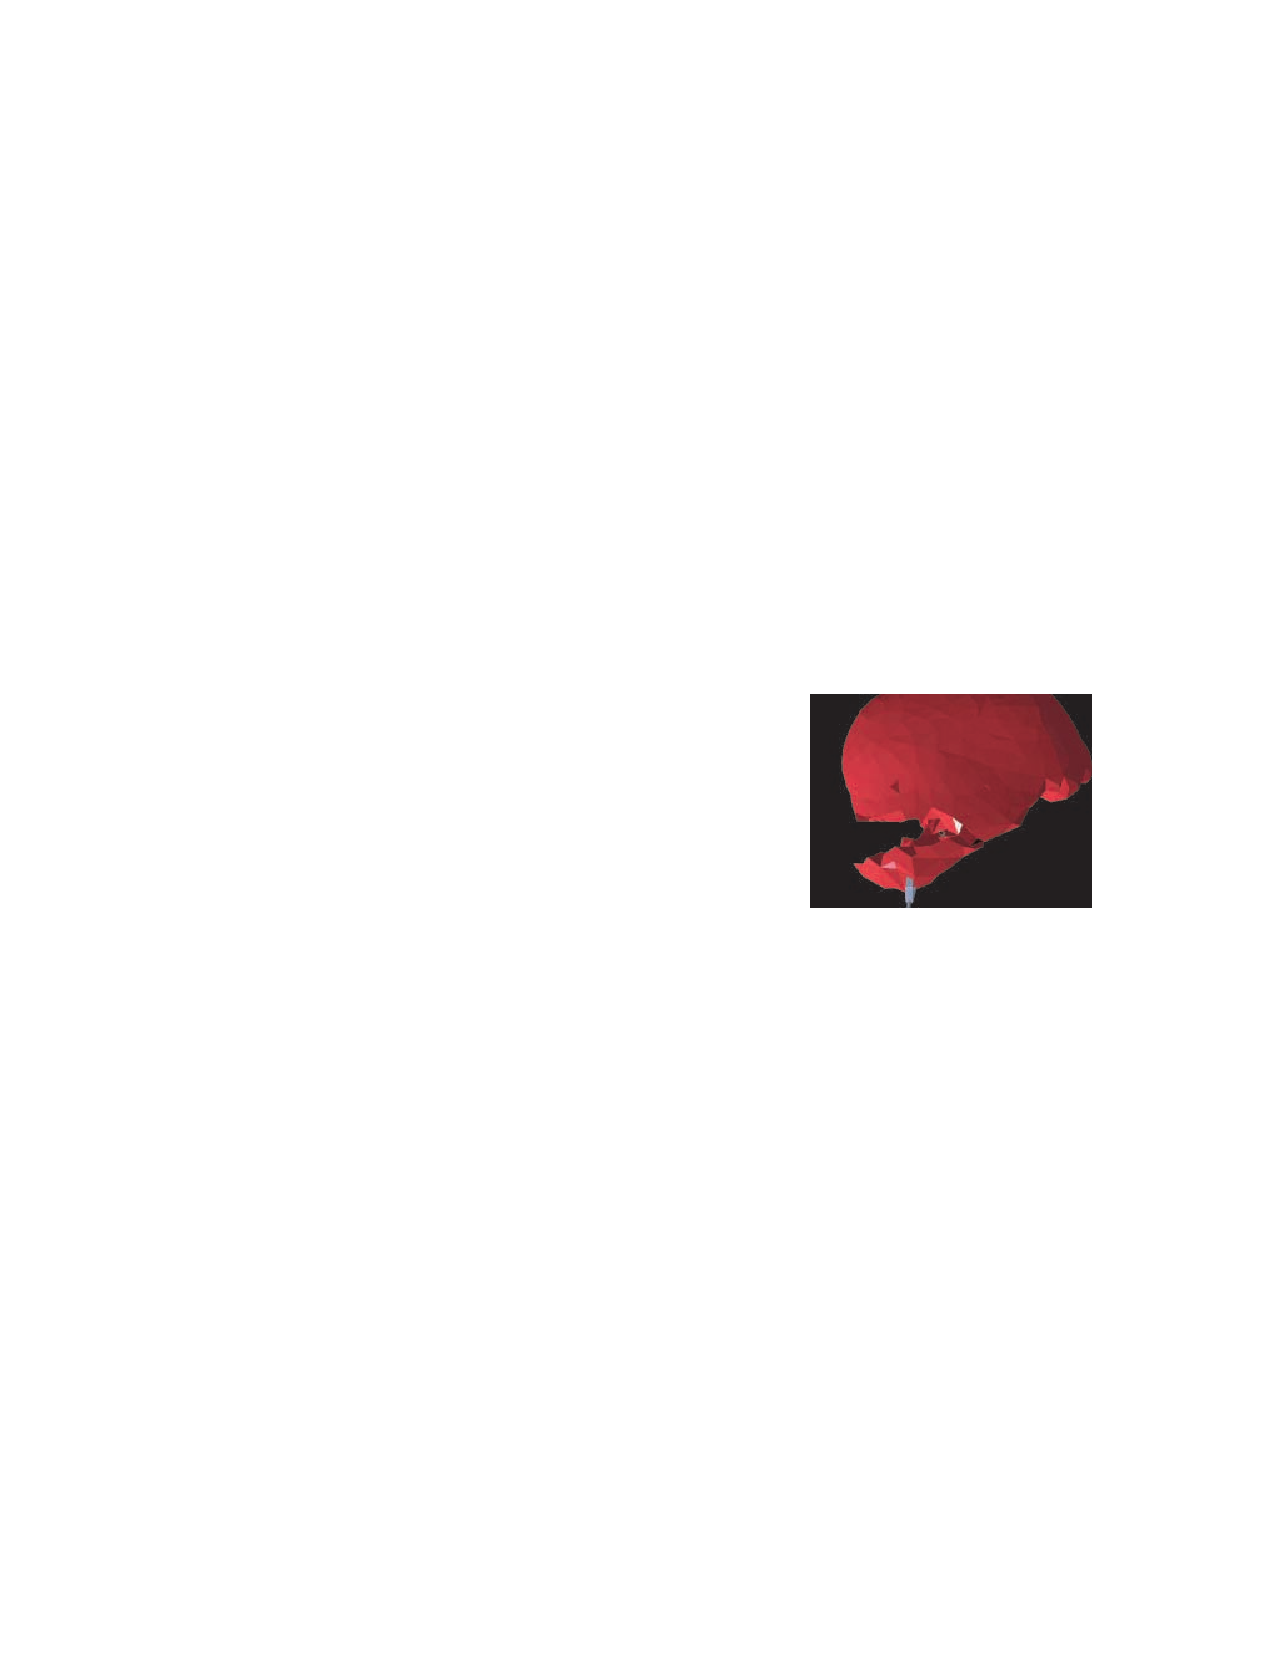
\includegraphics[height=4.5cm]{chapter4/hybrid2.pdf}
\end{center}
\caption[Simulation of a hepatectomy using a hybrid model]{Simulation of a hepatectomy using a hybrid model. $ 18 $\% of the mesh was modelled with the tensor-mass model (green) and therefore could be cut out. The rest of the mesh was simulated with the precomputed finite element model. } 
\label{chap4:fig-hybridModel}
\end{figure}

\cite{Serby01} described a new approach to cutting with finite element models. The central idea is not to introduce new nodes/elements but to displace the existing ones to account for the topological changes introduced by a cut. They also added a step of homogenisation of the mesh to avoid tiny elements. Thus, the problem of decreasing element size is minimised and consequently the stability of the solution of the equations of motion is increased. 

Cutting is a problem for all techniques precomputing the inverse of the stiffness matrix. Indeed, topological changes require updates of this matrix, which is too computationally heavy to be done in real-time. \cite{Nienhuys01} avoid the precomputations by approximating the inverse at runtime with an iterative algorithm (Conjugate Gradient). Moreover, instead of subdividing each tetrahedron to make the cut appear where the user performed it, they adapt the mesh locally so that there are always triangles on the scalpel path, and perform the cut along those triangles. If the approach is interesting, the authors reported a lag between the scalpel and the realised cut. In addition, repositioning the nodes within the mesh can easily generate degeneracies, which have to be eliminated. 
%
\begin{figure}[h]
\begin{center}
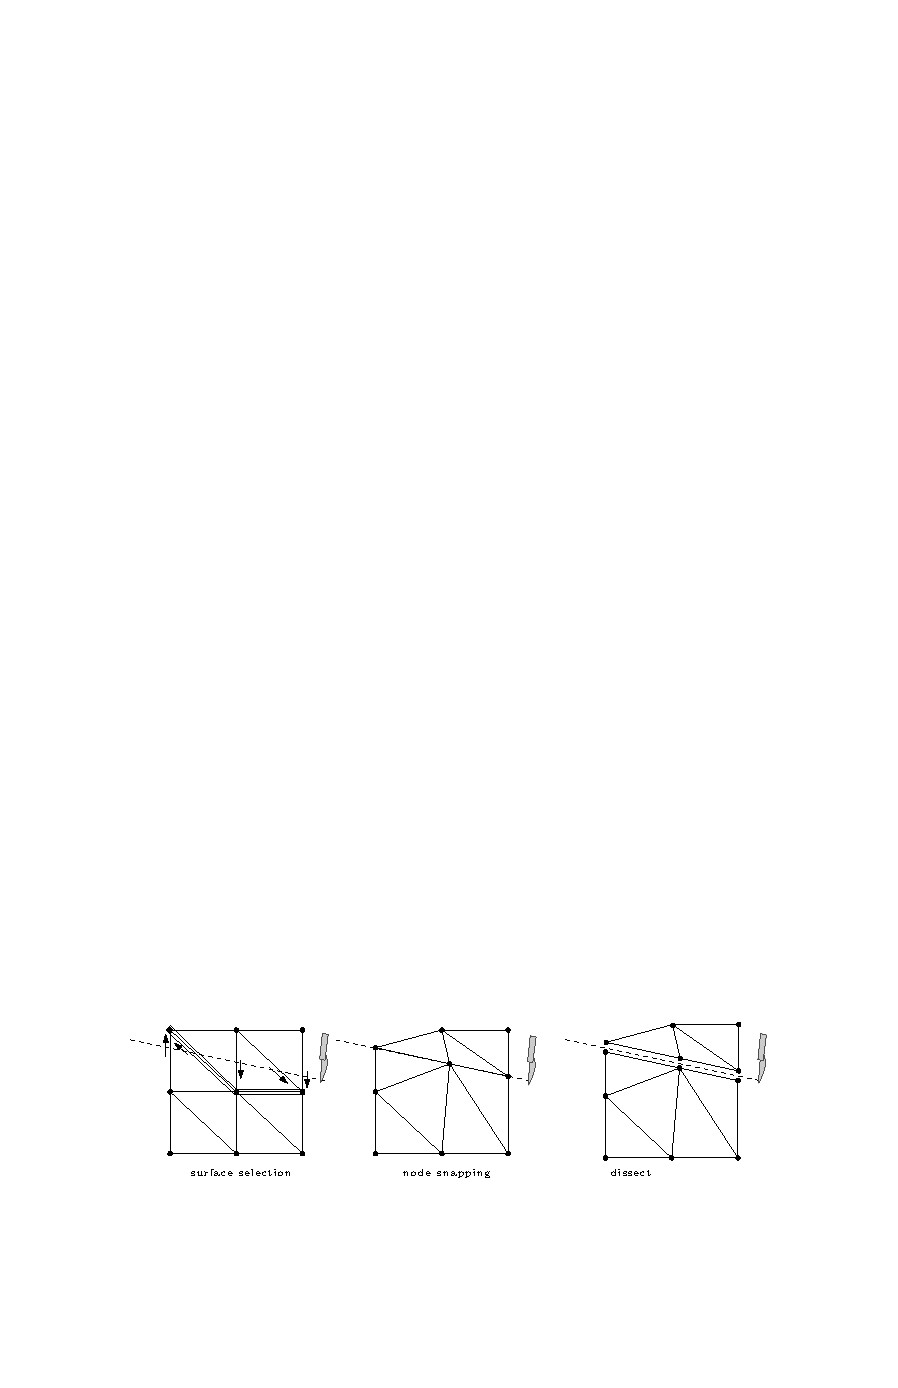
\includegraphics[width=13cm]{chapter4/cutUnderScalpel.pdf}
\end{center}
\caption[The three steps in performing a cut]{The three steps in performing a cut (represented here in 2D).} 
\label{chap4:fig-cutUnderScalpel}
\end{figure}

\bigskip

As we know, the assumption of linearity is usually only valid for very small deformations and strains. If this is often an acceptable trade-off between the visual deformation result and the speed of the system, research was carried out to handle large deformations. However, since geometrically non-linear analyses are highly computationally demanding, another approach was found which allows large deformation while still relying on a linear strain measure: the \emph{co-rotational} methods \label{chap4:corotationalMethods}. A very complete description of the co-rotational approach is given by \cite{Felippa00}. As explained in section~\ref{chap2:strainMeasures}, an appropriate strain measure is a tensor which only measures the deformation applied to the object. This is the case of the Cauchy-Green or Green tensors for instance. Those strain metrics only measures deformation, they are invariant with respect to rigid-body transformations applied. However, geometrically linear analyses make use of the infinitesimal strain tensor, which is only an approximation of the Green tensor. Consequently, this linearised strain measure is not invariant with respect to rigid-body transformations. In particular, the error brought by the approximated (linear) strain measure increases with the rotation of the element. This error in the measure creates ghost forces which overdeforms the simulated object. The idea behind co-rotational methods is the decomposition of the motion into a rigid-body and deformational components. In other words, the deformation of each element may be seen as measured in a coordinate system which follows the rigid-body motion of the element, hence cancelling the part of the error due to the rotation in the strain measure. Consequently, co-rotational formulations allow large displacements and rotations (since the rigid-body motion is not considered) as long as the strain remains small (the strain measure is still linear). 

Among the firsts to apply this technique to static analyses are \cite{Argyris64} and \cite{Wempner69}. Although the birth of co-rotational methods is not very clear \citep{Felippa05}, \cite{Belytschko73} had a similar thinking and introduced the so-called \emph{convected coordinates} for solving dynamic equations. However, while the spirit is the same than co-rotational methods, convected coordinates forms a curvilinear system that fits the change of metric as the body deforms, therefore the convected metric necessarily emcompasses deformations. In other words, the decomposition in rigid-body and deformational components is not exact. During the last decade, the co-rotational approach has regained interest in the computer graphics community. 

In constrast of \cite{Muller02} who discretised the rotation field at each vertex, \cite{Hauth04} determined the rotation at the level of the element. If \citeauthor{Muller02}'s technique of stiffness warping yields ghost forces due to inaccuracies in the determination of the rotation field, \citeauthor{Hauth04} made use of the polar decomposition of the deformation gradient to extract the exact rotation. They also applied this formulation in a hierarchical finite element setting where the coarse level is computed with a non-linear strain tensor and the finer levels are computed with a co-rotational method. In addition, they examined the error that is arising from using the co-rotational approximation instead of a non-linear strain tensor. They measured that the co-rotational approximation induces an error of about $5-20\,$\% but can give a speedup of about a factor seven or more. 

\cite{Pouliquen05} addressed the simulation of human fingers with haptic feedback. During the grasping task, the deformable finger pads undergo large rotations while their deformation remains small. Using a co-rotational approach for modelling the finger pads allows them to efficiently compute the contact forces between the deformable pads and the rigid object to be grasped. 

\bigskip

If co-rotational approaches increase accuracy in the strain measure, all the examples we have seen so far make use of a linear constitutive law. Yet, the mechanical behaviour of soft tissue is known to be non-linear, viscoelastic and often anisotropic \citep{Fung93}. Moreover, \cite{Misra07} demonstrated a noticeable difference between the force feedbacks provided by linear and non-linear tissue models. One of the first materially non-linear finite element formulation used in medical simulation was probably the work of \cite{Sagar94}. While developing a teleoperated micro-surgical robot for eye surgery, they wanted to provide a virtual environment has part of the system for training. Since the cornea is anisotropic and non-linearly elastic and undergoes large deformations, they have used large deformation elasticity theory with orthotropic and non-linear material properties in the finite element model. Coupled with a detailed visual model of the eye, the simulation produces a fair level of realism with a performance greater than $ 10 \,$Hz (see \fig{chap4:fig-eyeSurgery}). 
%
\begin{figure}[h]
\begin{center}
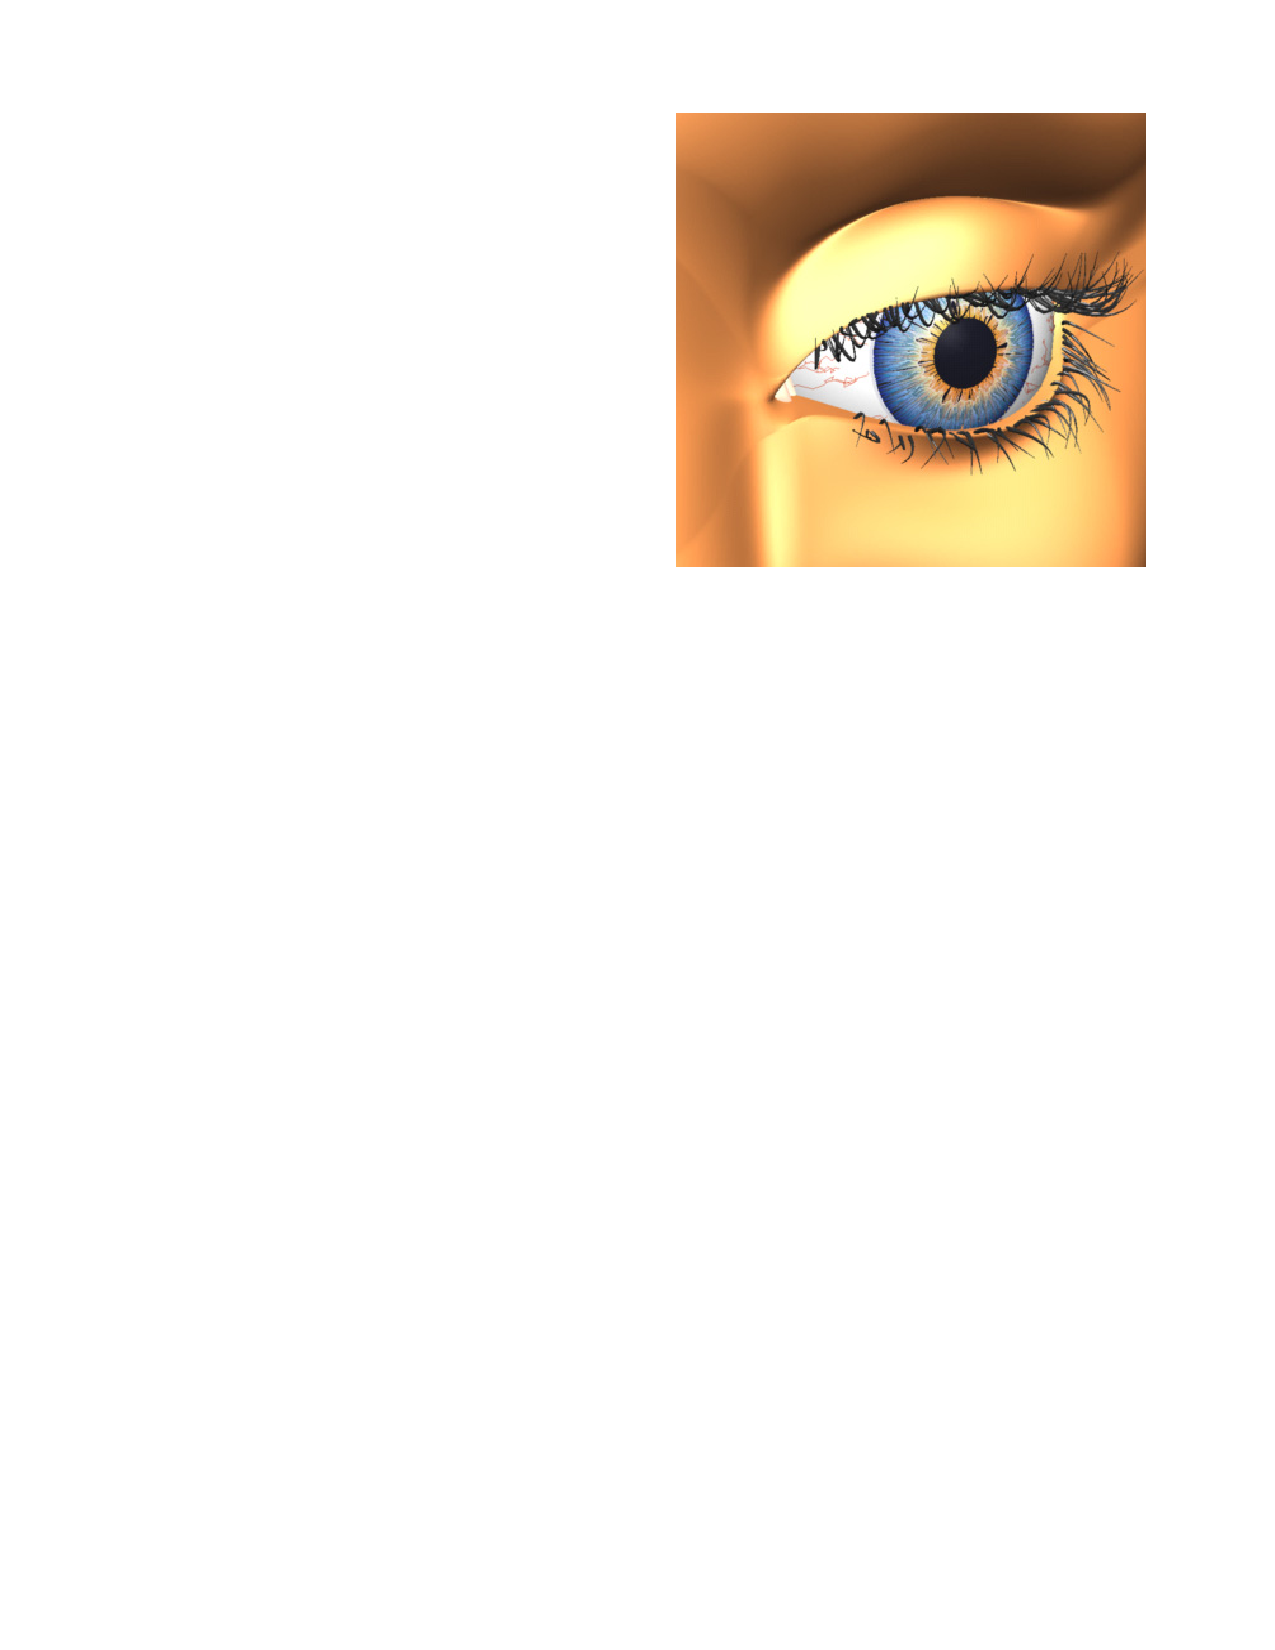
\includegraphics[height=5.5cm]{chapter4/eyeSurgery1.pdf}
\hspace{0.2cm}
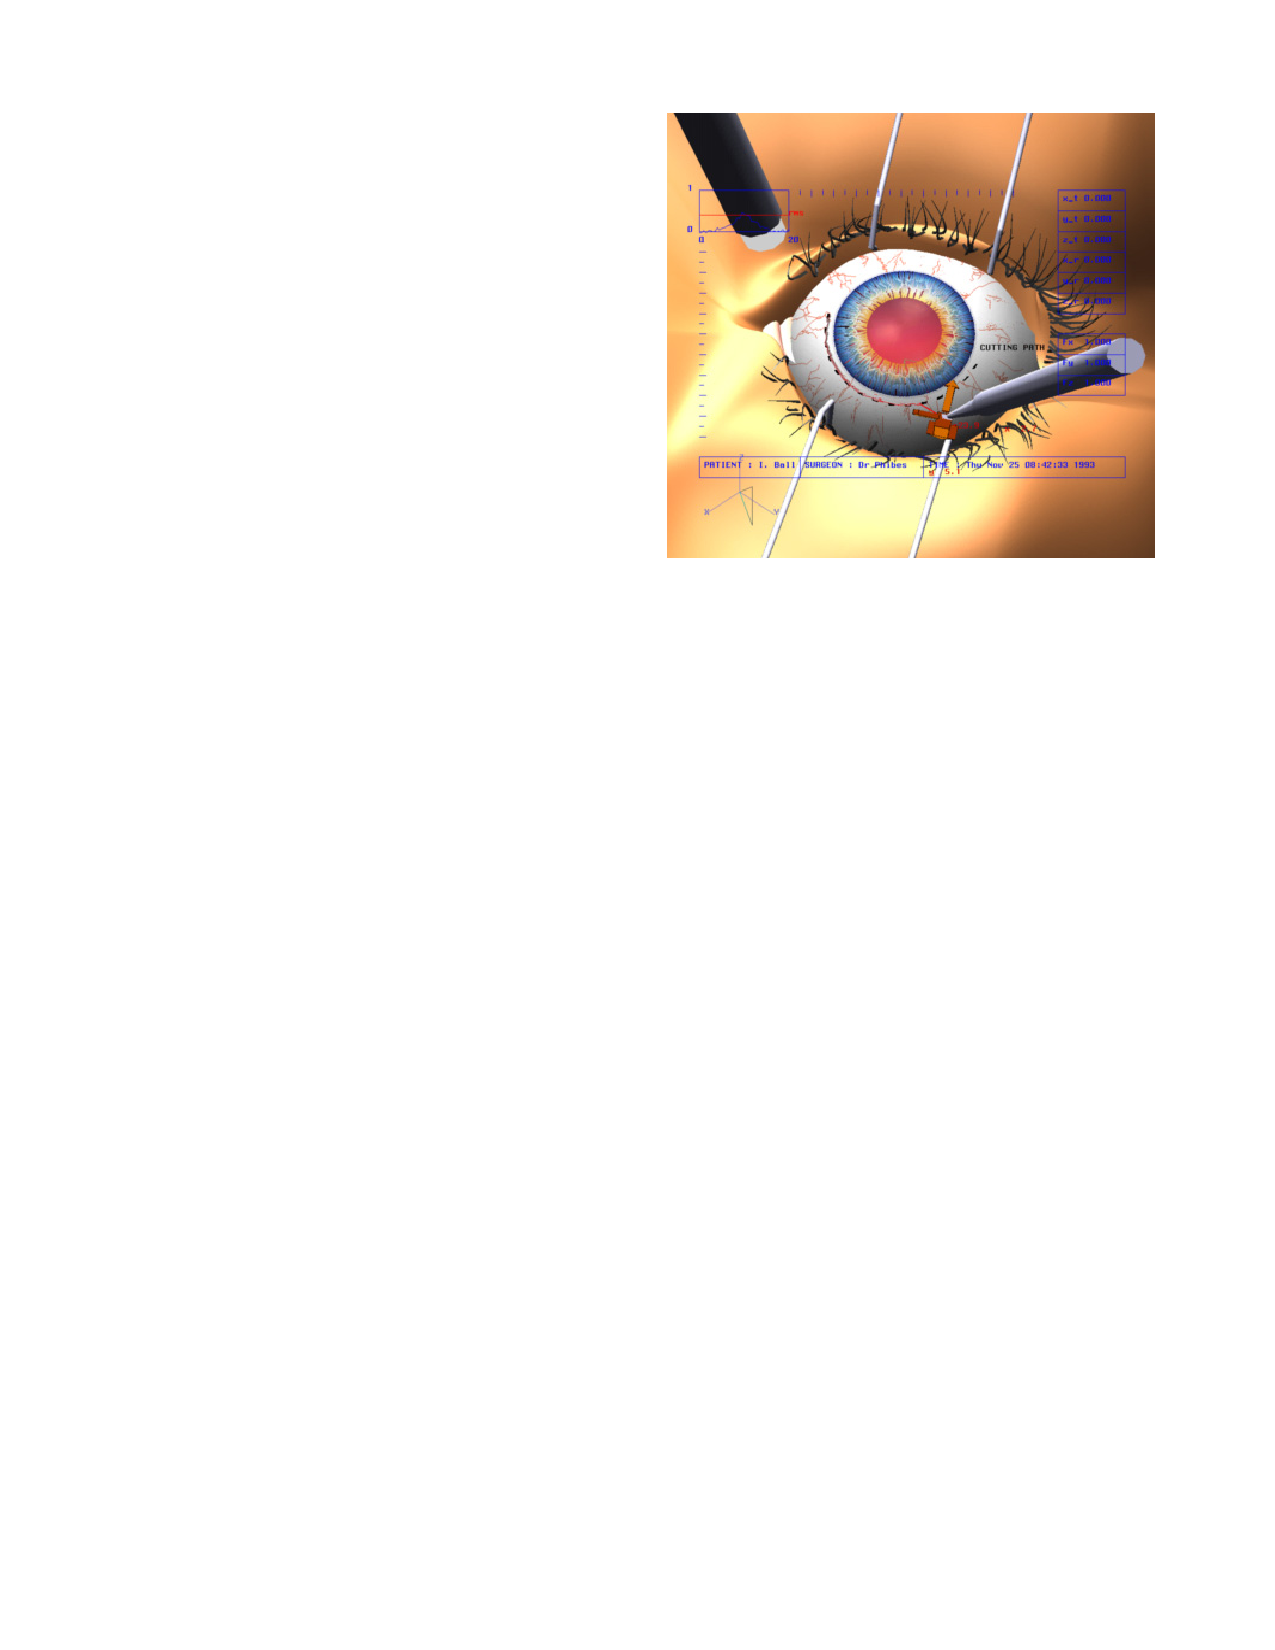
\includegraphics[height=5.5cm]{chapter4/eyeSurgery2.pdf}
\end{center}
\caption[Simulation of eye surgery]{(\textbf{Left}) Exterior view of the model showing the eye and the eyelashes. (\textbf{Right}) Surgical virtual environment including micro-tools and guidance information.} 
\label{chap4:fig-eyeSurgery}
\end{figure}

\cite{Keeve98} compared a fully (geometrically and materially) non-linear finite element model with a mass-spring model to compute the deformation of skin after bone realignment in a craniofacial surgery simulator. The efficiency of the mass-spring model gives the ability to the surgeon to realise interactive simulation of the resulting tissue changes and to improve his planning process. The best precision was given by the finite element model which could be used off-line to verify the chosen surgical procedure. 

The first geometrically non-linear finite element model running in real-time was reported by \cite{Debunne01}. They provided an adaptative method for animating viscoelastic deformable objects in a guaranteed frame rate. As the object moves and deforms, the sampling is refined to concentrate the computational load into the regions that deform the most (see \fig{chap4:fig-gummyBear}). They reported animating a few hundred points in real-time at a frequency higher than $ 300\,$Hz.
%
\begin{figure}[h]
\begin{center}
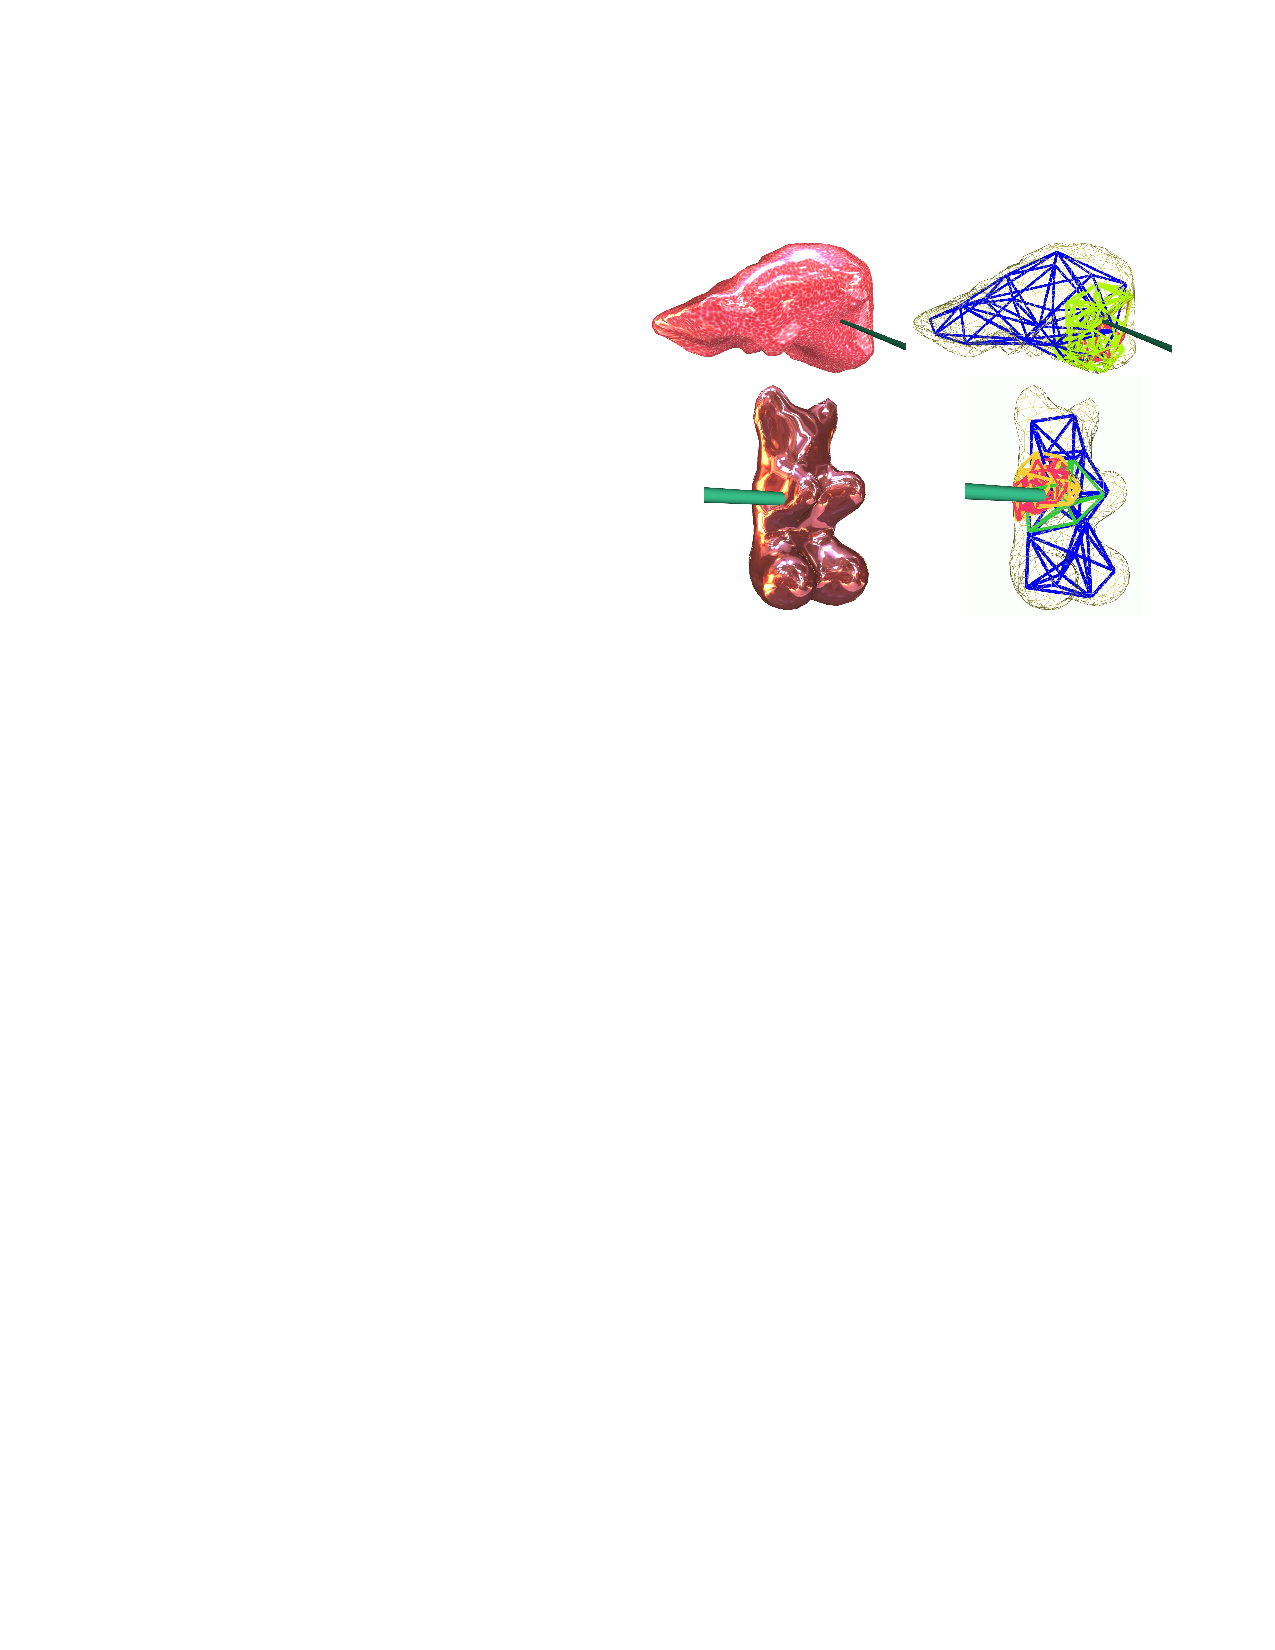
\includegraphics[width=13cm]{chapter4/gummyBear.pdf}
\end{center}
\caption[Simulation of a gummy bear]{The approach of \cite{Debunne01} makes use of a local refinement technique to ensure high physical fidelity while bounding the global computation load to guarantee real-time simulation with a geometrically non-linear and visco-elastic finite element model.} 
\label{chap4:fig-gummyBear}
\end{figure}

In the same spirit, \cite{Wu01} applied an adaptative meshing technique to provide sufficient detail where required while minimising unnecessary computation. They included both Mooney-Rivlin and Neo-Hookean material models and used the non-linear Cauchy-Green tensor. In addition to the local mesh refinement technique, they used mass lumping and an explicit time integration to deform a liver model of $ 1\,210 $ tetrahedra in real-time. 

Still in 2001, \citeauthor{Picinbono01} proposed to use a non-linear model only where the displacements are larger than a given threshold, the remaining part of the object still uses linear elasticity. 

Recently, research on non-linear finite element and more elaborate constitutive models increased significantly. For instance, \cite{Pathmanathan04} used a fully non-linear model to predict deformation of breast under compression during mammography. However, they were not interested in real-time. \cite{Zhong05} claimed achieving real-time with their non-linear finite element method using an interpolation approach but do not give any figure. \cite{Sedef06} proposed a viscoelastic model to simulate the deformation of a liver. They calculate the deformation in real-time by carrying out the computations in static and using the superposition principle. However, their approach used a linear strain measure, which limits their system to small deformations. \cite{Yan07} claimed to compute their non-linear finite element model in real-time using a technique of \emph{graded mesh} but do not give any information on their performance. 

In 2007, \citeauthor{Miller07} proposed the total Lagrangian explicit dynamics (TLED) algorithm, a very efficient fully non-linear formulation. The algorithm is based on the finite element method using the total Lagrangian formulation, where stresses and strains are measured with respect to the original configuration. This choice allows for precomputing of most spatial derivatives before the commencement of the time-stepping procedure. The authors reported that the average number of floating-point operations per element per time step is $35\, $\% lower than for the similar implementation of the algorithm based on updated Lagrangian formulation. They were able to compute the deformation of a hexahedral mesh of $ 6\,000 $ elements in about $ 16\,$ms for a time step of $ 1\,$ms. If they could not achieve real-time computations, their work constituted a step towards the simulation of entire organs in real-time. 

Finally, \cite{Taylor07a} presented an efficient constitutive update procedure for viscoelastic models suitable for simulation of soft tissues at large strains and varying strain rates. The procedure is formulated for use in explicit dynamic finite element algorithms like the TLED algorithm. The procedure is based on a class of visco-hyperelastic constitutive models developed from purely hyperelastic strain energy functions by introducing relaxation terms and expressing in convolution integral form. The resulting constitutive equations are separated into rate-dependent and -independent terms, with the former being designated as state variables to be stored and updated at each time step also. These are converted to a differential form, which upon integration in time yields the required incremental update formula. They showed the validity of the procedure with a series of numerical examples.

\bigskip

The finite element method is very computationally demanding. However, by nature, very similar computations are carried out for each element. Consequently, the finite element method is a good candidate for being implemented on parallel architectures. Thus, \cite{Szekely00} implemented a fully non-linear formulation for an 8-processor machine. However, the dedicated hardware was not yet assembled and functional at the time so they did not provide any measure of performance. 

Early 2000s, the rapid increase in the performance of graphics hardware, coupled with recent improvements in its programmability, have made graphics hardware a compelling platform for computationally demanding tasks in a wide variety of application domains. Researchers and developers have become interested in harnessing this power for general-purpose computing, an effort known collectively as GPGPU (for General-Purpose computing on Graphics Processing Units). A survey of GPGPU algorithms and techniques was written by \cite{Owens07}. 

To the best of our knowledge, \cite{Rumpf01} were the firsts to leverage the power of GPUs to solve partial differential equations. They established a correspondence between common mathematical operations and OpenGL operations and structures. Thus, as an example, a vector is represented as a RGBA color vector in a color image on the graphics card. They decided to implement an iterative solver for a linear system of equations, which we find at the core of most finite element codes. Using this hardware accelerated solver, they solved the linear heat equations and presented an anisotropic diffusion model for image processing. They obtained promising results but noted the hardware restrictions that forced them to approximate all non-linear functions by linear ones in the implementation of the anisotropic diffusion. Although a complete hardware accelerated finite element method implementation was yet to be done, \citeauthor{Rumpf01} definitely stepped towards the right direction. 

\cite{Wu04} proposed the first application of GPU in medical simulation \label{chap4:GPUMedicalSimulation}. They were able to achieve an interactive frame rate with topology changes in surgical simulation. Not only they used the condensation technique for merely calculating the surface nodes in the non-operation parts, but they implemented the conjugate gradient solver onto GPU. Indeed, entering 2003, the full IEEE floating point precision data type supported in shaders and texture stages allows the GPU to be applied into more general applications. The conjugate gradient solver includes three primary operations: multiplication of the sparse matrix and the vector, addition of two vectors and the sum-reduction operation. The core component is the multiplication of the sparse matrix and the vector. Therefore, they migrated this part of calculation from the CPU into the fragment processor of the GPU, to take advantage of the fragment processor in its efficient manipulation of the local texture memory on the mathematical calculation. The performance of their method on the GPU is up to $ 2.15 $ times faster than the CPU implementation. 

In 2007, \citeauthor{Taylor07b} introduced the first GPU implementation of a fully non-linear finite element method (more details in \cite{Taylor08}). They reformulated the TLED algorithm presented by \cite{Miller07} to accomodate with the limited hardware possibilities of GPUs. In particular, the main restriction when using graphics-based GPU execution is the inability to scatter, which necessitated reformulation of force summation as a gather in their implementation. It is worth noting that the entire finite element method implementation was ported to GPU. They reported significant solution speed gains up to $ 16.8 \times$ over the CPU implementation. Thus, they were able to compute a simple cube model with up to $ 16\,000 $ tetrahedral elements in real-time. 

	
	\subsection{Meshless methods}
	
If the finite element method is a robust method and widely used in engineering, the method has a few shortcomings \citep{Liu05}. First, the creation of a mesh is compulsory and producing a good quality mesh is both difficult and time consuming. Second, the stresses obtained in FEM are often discontinuous at the interfaces of the elements. Special techniques are required in a post-processing stage to recover accurate stresses. In addition, under large deformations, considerable loss in accuracy in FEM results can arise from the element distortions. The origin of these problems is the use of elements. Consequently, the idea of getting rid of the elements and the mesh has emerged and the concept of \emph{meshless} methods was born. Instead, meshless methods use a set of nodes scattered within the problem domain. They do not form a mesh, meaning it does not require any a priori information on the relationship between the nodes for the interpolation of the unknown variables. In theory, this should facilitate topological changes, a feature fairly desirable in surgery simulation. It is worth noting though that meshless methods are still in their developing stage and are not as mature as finite element formulations. We will now briefly review the research carried out in soft tissue modelling for medical simulation that makes use of meshless method. A complete review and details on meshless methods are beyond the scope of this thesis. 

\bigskip

A meshless method was introduced for the first time for modelling soft tissue in medical simulation by \cite{De01}. They use the so-called method of finite spheres (MFS). Nodal points are only sprinkled locally around the surgical tool tip and not over the whole domain. The interpolation is performed by functions that are nonzero only on spheres surrounding the nodes. A point collocation technique is used to generate the discrete equations. The authors qualitatively compared the method of finite spheres with the finite element technique from a commercial package and the displacement profil was similar in both cases. They were able to achieve a computational rate of about $ 100\, $Hz when 34 spheres where used. Real-time haptic rates of about $ 1\, $kHz was then obtained using a force extrapolation technique.

\cite{Lim04} used the same technique of finite spheres introduced by \citeauthor{De01} to model soft tissue but they added progressive cutting, without the generation of new primitives. As the cut progresses, the nearest vertex to the intersection point of the tool is snapped to the tool path. Then, they observed that the prescribed boundary condition changes on only a very small portion as the tool interacts with the organ. Rather than solving the entire problem over and over again, they proposed instead to make incremental corrections, which results in an accelerated solution procedure. 

Meshless methods were then introduced to computer graphics by \cite{Muller04}. In each step, they compute the spatial derivatives of the displacement field using a moving least squares (MLS) procedure. From these derivatives, they obtain strains, stresses and elastic forces at each simulated point. In addition, they proposed techniques for modelling and animating a point-sampled surface that dynamically adapts to deformations of the underlying volumetric model. They used a non-linear measure of strain with a linear constitutive model. They reported real-time simulation of models exibiting elastic, plastic, melting and flowing effects. 

\cite{Horton06} tested meshless methods for surgical simulation. They proposed a total Lagrangian explicit dynamics algorithm using a non-linear material formulation. They applied the method on an example of brain shift and compared their results with a commercial finite element code. The shape functions are created from a cloud of unconnected nodes using the element free Galerkin method. They were interested in the displacement of the centre of mass for the brain and found the absolute displacement differences between the two algorithm are less than $ 0.85\,$mm which is the resolution of the MRIs in their study. The same team kept investigating and testing the technique. However, they used moving least squares procedure for creating the shape functions instead of the element free Galerkin method. They also realised experimental indentations \citep{Horton07} and provided more extensive comparisons with a finite element method \citep{Horton10}.

Another example of application is the used of the technique called moving particule semi-implicit method (MPS) by \cite{Chhatkuli09}. They applied this method to simulate the deformation of lung and a tumor inside the left lung during inspiration. The lung tissues were considered to be homogeneous, isotropic and viscoelastic. They compared their results with the experimental CT taken at the end of inspiration and found out that the deformation predicted by numerical simulation matches reasonably well with the experimental results. 

\bigskip

\TODO{add drawbacks of meshless methods: supposedly good for handling topological changes but other issues. Couldn't really find drawbacks in meshless' literature.}